\documentclass{article}
\usepackage{multicol}
\usepackage{tocloft}
%%%%Sửa đường dẫn tới subsection,section
\usepackage[colorlinks=true, linkcolor=blue
  ,hypertexnames=false% <- added
]{hyperref}
%%%%Sửa đường dẫn tới subsection,section
\usepackage{colortbl}
\usepackage[export]{adjustbox}
\usepackage{marvosym}
\usepackage{comment}
\usepackage{accents}
\usepackage{diagbox}
\usepackage{helvet}
\usepackage{enumitem}
\usepackage{amssymb}
\usepackage{listings}
\usepackage{xcolor}
\definecolor{codegreen}{rgb}{0,0.6,0}
\definecolor{codegray}{rgb}{0.5,0.5,0.5}
\definecolor{codepurple}{rgb}{0.58,0,0.82}
\definecolor{backcolour}{rgb}{0.95,0.95,0.92}
\lstdefinestyle{mystyle}{
    %backgroundcolor=\color{backcolour},   
    commentstyle=\color{codegreen},
    keywordstyle=\color{magenta},
    numberstyle=\large\color{codegray},
    stringstyle=\color{codepurple},
    basicstyle=\ttfamily\large,
    breakatwhitespace=false,         
    breaklines=true,                 
    captionpos=b,                    
    keepspaces=true,                 
    numbers=left,                    
    numbersep=10pt,                  
    showspaces=false,                
    showstringspaces=false,
    showtabs=false,                  
    tabsize=2
}
\lstset{style=mystyle}
\usepackage{tikz}
\usetikzlibrary{calc}
\usepackage{tikz,tkz-tab}
\usepackage[utf8]{vietnam}
\renewcommand\thepart{\Alph{part}}
\renewcommand\thesection{\Roman{section}}
\renewcommand\thesubsection{\arabic{subsection}}
\usepackage{titlesec}
\titleformat*{\section}{\fontsize{20pt}{0pt}\selectfont \bfseries }
\usepackage{graphicx}
\usepackage{wrapfig}
\usepackage{float}
\usepackage{geometry}
\usepackage{fancyhdr}
\usepackage[framemethod=TikZ]{mdframed}
\usepackage{amsthm}
\geometry{a4paper,total={170mm,257mm},left=20mm,top=20mm,}
\usepackage{xcolor} 
\pagestyle{fancy} % header & footer
\fancyhf{} %xóa tất cả l c r head foot
\lhead{ĐSTT - L07 - 13} % đầu trái
\rfoot{Trang \thepage} %chân phải
\renewcommand{\headrulewidth}{1pt} % độ dày line
\renewcommand{\footrulewidth}{1pt}
\setcounter{secnumdepth}{4} % đếm số cho Heading 4 (1.1.1.1)
\setcounter{tocdepth}{4}
% HEADING 1
\titlespacing*{\section}{0pt}{0pt}{30pt} % a3 là d từ section tới dòng đầu tiên, a1 là d của sec so với lề trái
\titleformat*{\section}{\fontsize{16pt}{0pt}\selectfont \bfseries \centering} % a1 là size sec, a2 là d sec so với đầu trang 
%HEADING 2
\titlespacing*{\subsection}{0pt}{10pt}{10pt} 
\titleformat*{\subsection}{\fontsize{14pt}{0pt}\selectfont \bfseries}
% HEADING 3
\titlespacing*{\subsubsection}{0pt}{10pt}{10pt} 
\titleformat*{\subsubsection}{\fontsize{13pt}{0pt}\selectfont \bfseries \itshape  }
% HEADING 4
\titlespacing*{\paragraph}{0pt}{10pt}{0pt} 
\titleformat*{\paragraph}{\fontsize{11pt}{0pt}\selectfont \bfseries \itshape }
% Câu lệnh và các thư viện để chỉnh CAPTION
\renewcommand{\figurename}{\fontsize{13pt}{0pt}\selectfont \bfseries Hình}

\renewcommand{\thefigure}{\thesection.\arabic{figure}}
\usepackage{caption}
\captionsetup[Figure]{labelsep=space}

\renewcommand{\tablename}{\fontsize{13pt}{0pt}\selectfont \bfseries Table}
\renewcommand{\thetable}{\thesection.\arabic{table}}
\captionsetup[table]{labelsep=space}

\renewcommand{\theequation}{\thesection.\arabic{equation}}
%%%%%%%%%%%%%% Font chữ %%%%%%%%%%%%
\renewcommand{\familydefault}{\rmdefault}
%%%%%%%% Hyperref %%%%%%%%%%
\usepackage{hyperref}
\hypersetup{
    colorlinks=true,
    linkcolor=blue,
    filecolor=magenta,      
    urlcolor=cyan,
    pdftitle={Overleaf Example},
    pdfpagemode=FullScreen,
    }
\urlstyle{same}
%%%%%%%%%%%
\usepackage{mathtools}
\usepackage{bm}
\usepackage{esvect}
\title{\textbf{ĐẠI HỌC QUỐC GIA TP. HỒ CHÍ MINH}}
\author{\textbf{Trường Đại học Bách Khoa}}
\date{Khoa khoa học và kỹ thuật máy tính}


%%%%%%%%%%%%%%%%%%%%%%%%%%%%%%%%%%%%%%%%%%%%%%%
\newcounter{tongquat}[section] \setcounter{tongquat}{0}
\newenvironment{tongquat}[2][]{%
\refstepcounter{tongquat}%
\ifstrempty{#1}%
{\mdfsetup{%
frametitle={%
\tikz[baseline=(current bounding box.east),outer sep=0pt]
\node[anchor=east,rectangle,fill=blue!20]
{\strut Tổng quát};}}
}%
{\mdfsetup{%
frametitle={%
\tikz[baseline=(current bounding box.east),outer sep=0pt]
\node[anchor=east,rectangle,fill=blue!20]
{\strut Tổng quát};}}%
}%
\mdfsetup{innertopmargin=10pt,linecolor=blue!20,%
linewidth=2pt,topline=true,%
frametitleaboveskip=\dimexpr-\ht\strutbox\relax
}
\begin{mdframed}[]\relax%
\label{#2}}{\end{mdframed}}
%%%%%%%%%%%%%%%%%%%%%%%%%%%%%%%%%%%%%%%%%%%%%%%
%%%%%%%%%%%%%%%%%%%%%%%%%%%%%%%%%%%%%%%%%%%%%%%
\newcounter{chinhtac}[section] \setcounter{chinhtac}{0}
\newenvironment{chichtac}[2][]{%
\refstepcounter{chichtac}%
\ifstrempty{#1}%
{\mdfsetup{%
frametitle={%
\tikz[baseline=(current bounding box.east),outer sep=0pt]
\node[anchor=east,rectangle,fill=blue!20]
{\strut Chính tắc};}}
}%
{\mdfsetup{%
frametitle={%
\tikz[baseline=(current bounding box.east),outer sep=0pt]
\node[anchor=east,rectangle,fill=blue!20]
{\strut Chính tắc};}}%
}%
\mdfsetup{innertopmargin=10pt,linecolor=blue!20,%
linewidth=2pt,topline=true,%
frametitleaboveskip=\dimexpr-\ht\strutbox\relax
}
\begin{mdframed}[]\relax%
\label{#2}}{\end{mdframed}}
%%%%%%%%%%%%%%%%%%%%%%%%%%%%%%%%%%%%%%%%%%%%%%%
%%%%%%%%%%%%%%%%%%%%%%%%%%%%%%%%%%%%%%%%%%%%%%%
\newcounter{chuan}[section] \setcounter{chuan}{0}
\newenvironment{chuan}[2][]{%
\refstepcounter{chuan}%
\ifstrempty{#1}%
{\mdfsetup{%
frametitle={%
\tikz[baseline=(current bounding box.east),outer sep=0pt]
\node[anchor=east,rectangle,fill=blue!20]
{\strut Dạng chuẩn};}}
}%
{\mdfsetup{%
frametitle={%
\tikz[baseline=(current bounding box.east),outer sep=0pt]
\node[anchor=east,rectangle,fill=blue!20]
{\strut Dạng chuẩn};}}%
}%
\mdfsetup{innertopmargin=10pt,linecolor=blue!20,%
linewidth=2pt,topline=true,%
frametitleaboveskip=\dimexpr-\ht\strutbox\relax
}
\begin{mdframed}[]\relax%
\label{#2}}{\end{mdframed}}
%%%%%%%%%%%%%%%%%%%%%%%%%%%%%%%%%%%%%%%%%%%%%%%

\begin{document}

\begin{titlepage}
    \begin{tikzpicture}[overlay, remember picture]
\draw[line width=3pt]
    ($ (current page.north west) + (2.0cm,-2.0cm)$)
    rectangle
    ($ (current page.south east) + (-2.0cm,2.5cm)$);
\draw[line width=2pt]
    ($ (current page.north west) + (2.2 cm,-2.2cm)$)
     rectangle
    ($ (current page.south east) + (-2.2cm,2.7cm)$);

\end{tikzpicture}
\begin{center}
\vspace{1pt} {\large {BỘ GIÁO DỤC VÀ ĐÀO TẠO}} \\
\textbf{\fontsize{14pt}{0pt}\selectfont  ĐẠI HỌC QUỐC GIA THÀNH PHỐ HỒ CHÍ MINH }\\
\textbf{\fontsize{14pt}{0pt}\selectfont  TRƯỜNG ĐẠI HỌC BÁCH KHOA }\\
\rule{0.5\textwidth}{1pt}

\begin{figure}[h]
    \centering
    
\includegraphics[scale=0.4]{01_logobachkhoa.png}
\end{figure}
\vspace{1pt}
\fontsize{18pt}{0pt}\selectfont BÁO CÁO \\
\vspace{1pt}
\textbf{\fontsize{20pt}{0pt}\selectfont BỘ MÔN ĐẠI SỐ TUYẾN TÍNH}\\
\vspace{0.5cm}
\underline
{\fontsize{16pt}{1pt} \selectfont \textbf{Đề tài 13:}}
\end{center}
\begin{center}
    %{\fontsize{30pt}{1pt}\selectfont \textbf {RATES OF CHANGE IN THE NATURAL AND SOCIAL SCIENCE}}
    \parbox[t][][c]{5.5in}{\centering \fontsize{24pt}{1pt} \selectfont  \textbf {QUY HOẠCH TUYẾN TÍNH}} \\ 
\end{center}
\begin{center}
\vspace{0.5cm}
    \begin{tabular}{|w{l}{3.5cm}|p{5.75cm}|}
    \hline
        MSSV & Họ và tên \\
        \hline
        2311070 & Nguyễn Xuân Huy Hoàng \\
        2310795 & Phạm Anh Đức \\
        2311694 & Phạm Đăng Khôi \\
        2311635 & Phạm Đặng Đăng Khoa \\
        2310761 & Phạm Đình Được \\
        2312186 & Phạm Đình Phương Nam \\
        2310686 & Phạm Đỗ Thành Đạt \\
        \hline
\end{tabular}
\end{center}
\begin{center}
    \textbf {
    Giảng viên hướng dẫn: Ts.Nguyễn Thị Hoài Thương \\
    Nhóm: ĐSTT-L07-13}
\end{center}
\begin{center}
    \vspace{1cm}
    \large \textbf{Ngày 10 tháng 3 năm 2024}
\end{center}
\end{titlepage}

\thispagestyle{empty}
\addtocontents{toc}{\protect\thispagestyle{empty}}
\clearpage
\thispagestyle{empty}
\addtocontents{toc}{\protect\thispagestyle{empty}}
\tableofcontents
\thispagestyle{empty}
\clearpage
\large


\newpage
\phantomsection
\clearpage
\section*{I. KHÁI NIỆM}
\addcontentsline{toc}{section}{\protect\numberline{}I. KHÁI NIỆM}
\setcounter{section}{1}\setlength{\baselineskip}{15pt}
   % đếm số cho section2, nếu không là hiện 0.1, 0.1.1
\setcounter{subsection}{0}
\setcounter{subsubsection}{0}
\large
\pagenumbering{arabic} % đánh số thứ tự 1,2,3,4,.....

\subsection{Quy hoạch tuyến tính}
%\addcontentsline{toc}{subsection}{\numberline{}Quy hoạch tuyến tính}
\large

\hspace{0.4cm} \textit{Quy hoạch tuyến tính} - linear programming (LP) là một thuật toán nhằm tìm ra phương án tối ưu (hoặc kế hoạch tối ưu) từ vô số các phương án quyết định. Phương án tối ưu là phương án thoả mãn được các mục tiêu đề ra của một hãng, phụ thuộc vào các hạn chế và các ràng buộc.\medskip \\ 
\indent Thuật toán LP đề cập đến vấn đề phân bổ nguồn lực khan hiếm giữa các hoạt động cạnh tranh trong một phương án tối ưu để đạt được hiệu quả cao nhất, lãi gộp cao nhất hay doanh thu hoặc chi phí thấp nhất. Mô hình quy hoạch tuyến tính gồm \textit{2 thành phần cơ bản}:\\
\begin{itemize}
    \item [$\square$] \textbf{Hàm mục tiêu:} Biểu thị giá trị mà ta muốn tối ưu hóa (tối đa hóa hoặc tối thiểu hóa) để đạt được mục tiêu cụ thể.
    \item [$\square$] \textbf{Điều kiện ràng buộc:} Các ràng buộc dưới dạng các hạn chế về sự sẵn có của nguồn lực hay thoả mãn các yêu cầu tối thiểu.
\end{itemize}
$\hookrightarrow$ Do đó có thể hiểu đơn giản quy hoạch tuyến tính là lĩnh vực toán học nghiên cứu các bài toán tối ưu mà hàm mục tiêu (vấn đề được quan tâm) và các ràng buộc (điều kiện của bài toán) đều là hàm và các phương trình hoặc bất phương trình tuyến tính.

\subsection{Một số khái niệm khác liên quan}
%\addcontentsline{toc}{subsection}{\numberline{}4. Một số khái niệm khác liên quan}
\begin{itemize}
    \item [$\square$] \textbf{Biến quyết định:} Các biến đại diện cho các hoạt động hoặc quyết định trong bài toán.
    \item [$\square$] \textbf{Biến slack và surplus:} Các biến được thêm vào một số ràng buộc để biến đổi chúng thành dạng chuẩn tắc.
    \item [$\square$] \textbf{Phương án:} Mỗi vector $X=(x_1,x_2,...,x_n)$ trong $R^n$ thỏa mãn tất cả các ràng buộc của một bài toán quy hoạch tuyến tính $n$ biến được gọi là một phương án của bài toán đó.
    \item [$\square$] \textbf{Tập phương án (hay miền ràng buộc):} Tập hợp tất cả các phương án của một bài toán quy hoạch tuyến tính gọi là tập phương án hay miền ràng buộc của bài toán đó.
    \item [$\square$] \textbf{Phương án tối ưu:} Một phương án $x^*$ của bài toán quy hoạch tuyến tính được gọi là nghiệm hay là phương án tối ưu nếu nó làm cho hàm mục tiêu đạt $min$ (hoặc $max$) đúng như yêu cầu bài toán đó.
    \item [$\square$] \textbf{Phương án cực biên}
        \begin{itemize}[label=\textbullet]
            \item \textbf{Đối với bài toán quy hoạch tuyến tính dạng tổng quát:} Xét một bài toán quy hoạch tuyến tính dạng tổng quát có $n$ biến $x_1, x_2,...,x_n$. Một phương án $x^* =(x^*_1, x^*_2,...,x^*_n) $ của bài toán quy hoạch tuyến tính dạng tổng quát đang xét được gọi là \textbf{phương án cực biên} nếu nó thỏa mãn dấu $"="$ (còn gọi là thỏa mãn chặt) với ít nhất $n$ ràng buộc trong đó có đúng $n$ ràng buộc độc lập tuyến tính (tức là ma trận hệ số của $n$ ràng buộc đó có hạng bằng $n$) trong hệ ràng buộc của bài toán quy hoạch tuyến tính dạng tổng quát.
            \item \textbf{Đối với bài toán quy hoạch tuyến tính dạng chính tắc hoặc chuẩn chính tắc:} Xét một bài toán quy hoạch tuyến tính dạng chính tắc có $n$ biến $x_1, x_2,...,x_n$. Một phương án $x^* =(x^*_1, x^*_2,...,x^*_n) $ của bài toán quy hoạch tuyến tính dạng chính tắc đang xét là \textbf{phương án cực biên} nếu hệ các cột ma trận hệ số ứng với các $x^*_j > 0$ lập thành hệ độc lập tuyến tính. Ta gọi các ẩn dương là ẩn cơ sở, các ẩn triệt tiêu là ẩn phi cơ sở. Các hệ số trong hàm mục tiêu ứng với các ẩn cơ sở (tương ứng, phi cơ sở) cũng được gọi là hệ số cơ sở (tương ứng, phi cơ sở). 
        \end{itemize}
    \item [$\square$] \textbf{Khái niệm điểm cực trị:}
    \begin{itemize}[label=\textbullet]
        \item Một điểm cực trị của một hàm mục tiêu trong bài toán quy hoạch là một điểm trong miền khả thi mà tại đó giá trị của hàm mục tiêu đạt cực đại hoặc cực tiểu.
        \item Các điểm cực trị thường nằm tại các giao điểm của các đường ràng buộc trong miền khả thi.
    \end{itemize}
    \item [$\square$] \textbf{Định lý về các điểm cực trị:}
    \begin{itemize}[label=\textbullet]
        \item Định lý về các điểm cực trị khẳng định rằng một bài toán quy hoạch có nghiệm tối ưu (hoặc cực tiểu) khi và chỉ khi nó có một nghiệm cơ bản khả thi tối ưu (hoặc cực tiểu).
        \item Định lý này là nền tảng cho phương pháp Simplex, vì nó cho phép chúng ta tìm kiếm nghiệm tối ưu bằng cách khảo sát từ nghiệm khả thi này sang nghiệm khả thi khác.
    \end{itemize} 
    \item [$\square$] \textbf{Bảng Simplex:} Một bảng được sử dụng để theo dõi tiến trình của quy trình Simplex và ghi lại thông tin về các biến, ràng buộc và giá trị hàm mục tiêu tại mỗi bước.
    \item [$\square$] \textbf{Quy trình Simplex:}
    \begin{itemize}[label=\textbullet]
        \item Quy trình Simplex bắt đầu với một nghiệm cơ bản khả thi bất kỳ.
        \item Tại mỗi bước, quy trình xác định một biến \textbf{vào} và một biến \textbf{ra} để di chuyển đến nghiệm cơ bản khả thi tiếp theo.
        \item Biến vào được chọn là biến có hệ số âm lớn nhất trong hàm mục tiêu tại nghiệm khả thi hiện tại.
        \item Biến ra được chọn là biến có tỷ lệ rẽ nhỏ nhất khi tính toán cho tất cả các ràng buộc.
        \item Quy trình tiếp tục cho đến khi tìm thấy nghiệm khả thi tối ưu hoặc xác định rằng bài toán quy hoạch không có nghiệm tối ưu.
    \end{itemize}
\end{itemize}
\subsection{Một số nhận xét quan trọng}
%\addcontentsline{toc}{subsection}{\numberline{}5. Một số nhận xét quan trọng}
\begin{itemize}
    \item [$\square$] Một bài toán quy hoạch tuyến tính có thể \textbf{không có phương án}, lúc đó nó \textbf{vô nghiệm}. Điều kiện cần và đủ để một bài toán quy hoạch tuyến tính có \textbf{phương án tối ưu} là nó có \textbf{phương án} và \textbf{hàm mục tiêu bị chặn}.
    \item [$\square$] Nếu bài toán quy hoạch tuyến tính có \textbf{phương án tối ưu} và có \textbf{phương án cực biên} thì chắc chắn có \textbf{phương án cực biên tối ưu}. Khi đó, ta chỉ cần tìm nghiệm trong các \textbf{phương án cực biên}.
    \item [$\square$] Bài toán quy hoạch tuyến tính dạng tổng quát luôn có \textbf{một số hữu hạn phương án cực biên}.
    \item [$\square$] Đối với bài toán quy hoạch tuyến tính dạng chính tắc chuẩn, ta luôn dễ dàng tìm được một \textbf{phương án cực biên} bằng cách cho các ẩn ứng với các hệ số không thuộc ma trận con sơ cấp là ẩn phi cơ sở, tức là gán cho chúng giá trị bằng 0. Các ẩn ứng với các hệ số thuộc ma trận con sơ cấp là các ẩn cơ sở.
\end{itemize}
\newpage
\subsection{Bài toán thực tế:}
\subsubsection{Bài toán sản xuất}
% \textbf{\underline{Bài toán:}} Một xí nghiệp cần sản xuất 3 loại bánh: bánh đậu xanh, bánh thập cẩm và bánh dẻo. Lượng nguyên liệu đường, đậu cho một bánh mỗi loại, lượng dự trữ nguyên liệu, tiền lãi cho một bánh mỗi loại được cho trong bảng sau:
% \newpage
% \begin{table}[tbh!]
% \large
%     \centering
%     \begin{tabular}{|c|c|c|c|c|}
%        \hline
%         Nguyên liệu &Bánh đậu xanh &Bánh thập cẩm &Bánh dẻo &Lượng dự trữ \\ \hline
%         Đường &0,04kg &0,06kg& 0,05kg &500kg \\ \hline
%         Đậu &0,07kg &0kg &0,02kg &300kg \\ \hline
%         Lãi &3000 &2000 &2500 \\ \hline
%     \end{tabular}
% \end{table}
% Hãy lập mô hình bài toán tìm số lượng mỗi loại bánh cần sản xuất sao cho không bị động về nguyên liệu mà lãi đạt được cao nhất.
\textbf{\underline{Bài toán:}} Từ $m$ loại nguyên liệu hiện có người ta muốn sản xuất $n$ loại sản phẩm nhằm thu được lợi nhuận cao nhất.\medskip \\
\indent Ta tiến hành mô hình hoá bài toán:\medskip \\
\indent Giả sử:
\begin{itemize}
    \item $a_{ij}$ là lượng nguyên liệu loại $i$ dùng để sản xuất 1 sản phẩm loại $j$ với $(i=1,2,...,m)$ và $(j=1,2,...,n)$
    \item $b_i$ là số lượng nguyên liệu loại $i$ hiện có.
    \item $c_j$ là lợi nhuận thu được từ việc sản xuất một đơn vị sản phẩm loại $j$.
\end{itemize}
\hspace{0.4cm} Vấn đề đặt ra là phải sản xuất mỗi loại sản phẩm là bao nhiêu sao cho tổng lợi nhuận thu được từ việc bán các sản phẩm lớn nhất trong điều kiện nguyên liệu hiện có. \medskip \\
\indent Gọi $x_j \geq 0$ là số lượng sản phẩm thứ $j$ sẽ sản xuất $(j=1,2,...,n)$ \medskip \\
\indent Tổng lợi nhuận thu được từ việc sản xuất sản phẩm là:
\begin{equation*}
    f(x) =\sum_{j=1}^n c_jx_j = c_1x_1 + c_2x_2 + ... + c_nx_n
\end{equation*}
\indent Vì yêu cầu lợi nhuận thu được là cao nhất nên ta cần có:
\begin{equation*}
    \max{f(x)} =\sum_{j=1}^n c_jx_j = c_1x_1 + c_2x_2 + ... + c_nx_n
\end{equation*}
\indent Đây chính là hàm mục tiêu của bài toán!
\begin{itemize}
    \item Lượng nguyên liệu thứ $i=1 \longrightarrow m$ dùng để sản xuất sản phẩm thứ 1 là $a_{i1}x_1 $
    \item Lượng nguyên liệu thứ $i=1 \longrightarrow m$ dùng để sản xuất sản phẩm thứ 2 là $a_{i2}x_2 $
    \item ...
    \item Lượng nguyên liệu thứ $i=1 \longrightarrow m$ dùng để sản xuất sản phẩm thứ $n$ là $a_{in}x_n $
\end{itemize}
\hspace{0.4cm} Vậy lượng nguyên liệu thứ $i$ dùng để sản xuất là các sản phẩm là:
\begin{equation*}
    a_{i1}x_1 + a_{i2}x_2 +...+ a_{in}x_n 
\end{equation*}
Vì lượng nguyên liệu thứ  $i=1 \longrightarrow m$ dùng để sản xuất các loại sản phẩm không thể vượt quá lượng được cung cấp là $b_i$ nên :
\begin{equation*}
    a_{i1}x_1 + a_{i2}x_2 +...+ a_{in}x_n \leq b_i (i=1,2,...,m)
\end{equation*}
Vậy theo yêu cầu của bài toán ta có mô hình sau đây:
\begin{equation*}
    \max{f(x)} =\sum_{j=1}^n c_jx_j = c_1x_1 + c_2x_2 + ... + c_nx_n
\end{equation*}
\begin{center}
    $\begin{cases}
        a_{11}x_1 + a_{12}x_2 +...+ a_{1n}x_n \leq b_1 \\
        a_{21}x_1 + a_{22}x_2 +...+ a_{2n}x_n \leq b_2 \\
        ...\\ 
        a_{m1}x_1 + a_{m2}x_2 +...+ a_{mn}x_n \leq b_m \\
        x_j \geq 0, (j=1,2,...,n)
    \end{cases}$
\end{center}
% \subsubsection{Bài toán phân công lao động}
% \textbf{\underline{Bài toán:}} Một lớp học cần tổ chức lao động với hai loại công việc: xúc đất và chuyển đất. Lao động của lớp được chia làm 3 loại A, B, C, với số lượng lần lượt là 10, 20, 12. Năng suất của từng loại lao động trên từng công việc cho trong bảng dưới đây: \\
% \begin{table}[tbh!]
% \centering
% \large
% \begin{tabular}{|c|c|c|c|}
% \hline
% Lao động& A(10) & B(20) & C(12) \\
% \hline
% Xúc đất & 6 & 5 & 4 \\
% \hline
% Chuyển đất & 4 & 3 & 2 \\
% \hline
% \end{tabular}
% \end{table}\\
% Hãy tổ chức lao động sao cho có tổng năng suất lớn nhất.
\subsubsection{Bài toán vận tải:}
% Bài toán vận tải cân bằng thu phát có cấu trúc gồm: m trạm phát (nhà kho), n trạm thu (cửa hàng) với tổng cung – cầu bằng nhau. Ngoài ra, ta còn có thông tin về chi phí của tuyến đường đi (trên 1 đơn vị hàng hóa). Bài toán đòi hỏi mô tả việc gửi hàng để cho tổng chi phí vận chuyển là ít nhất.\medskip \\
% Tiêu chí chung để chọn lượng hàng và loại cột/hàng:
% \begin{equation*}
%     x_{ij}=min\{a_i; b_i\} = \begin{cases}
%         a_i \hspace{2cm} \text{ loại dòng } i, b_j=b_j-a_i \\
%         b_j \hspace{2cm} \text{ loại cột } j, a_i=a_i-b_j \\
%         a_i = b_j \hspace{1.13cm}  \text{ loại dòng $i$ cột $j$}
%     \end{cases}
% \end{equation*}
\textbf{\underline{Bài toán:}} Người ta cần vận chuyển hàng hoá từ $m$ kho đến $n$ cửa hàng bán lẻ. Lượng hàng hoá ở kho $i$ là $s_i$ $(i=1,2,...,m)$ và nhu cầu hàng hoá của cửa hàng $j$ là $d_j$ $(j=1,2,...,n)$. Cước vận chuyển một đơn vị hàng hoá từ kho $i$ đến của hàng $j$ là $c_{ij} \geq 0$ đồng.\medskip \\
\indent Mô hình hoá bài toán:
\begin{itemize}
    \item Nhằm tối ưu hóa việc di chuyển hàng hóa từ các nguồn cung đến các điểm tiêu thụ một cách hiệu quả và có thể làm giảm chi phí vận chuyển nên hàm mục tiêu của bài toán là: 
    \begin{equation*}
        \min{f(x)} = \sum_{i=1}^m \sum_{j=1}^n c_{ij}x_{ij}
    \end{equation*}
    \item Để một phương án thực sự là chấp nhận được cho bài toán vận tải, các giá trị $\displaystyle x_{i,j}$ phải thỏa mãn các điều kiện ràng buộc
    \begin{itemize}
        \item Theo điều kiện về khả năng cung cấp:
        \begin{equation*}
            \sum_{j=1}^n x_{ij} = s_i \text{ với } (i=1,...,m)
        \end{equation*}
        \item Theo điều kiện về nhu cầu tiêu thụ:
        \begin{equation*}
            \sum_{i=1}^m x_{ij} = d_j \text{ với } (j=1,...,n)
        \end{equation*}
    \end{itemize}
    \item Điều kiện biên $x_{ij} \geq 0$ với $(i=1,...,m)$ và $(j=1,...,n)$
\end{itemize}
\hspace{0.4cm} Do đó ta có mô hình sau:
\begin{equation*}
        \min{f(x)} = \sum_{i=1}^m \sum_{j=1}^n c_{ij}x_{ij} \text{ }\text{ }\text{ }\text{ }
\end{equation*}
\begin{equation*}
    \begin{cases}
        \displaystyle \sum_{j=1}^n x_{ij} = s_i \text{ với } (i=1,...,m) \\
        \displaystyle \sum_{i=1}^m x_{ij} = d_j \text{ với } (j=1,...,n) \\
        \displaystyle x_{ij} \geq 0,(i=1,...,m); (j=1,...,n) \\
    \end{cases}
\end{equation*}
\subsubsection{Bài toán khẩu phần ăn:}
Một khẩu phần thức ăn có khối lượng P, có thể được làm từ $n$ loại thức ăn. Giá mua một đơn vị thức ăn loại $j$ là $c_j$. Để đảm bảo cơ thể phát triển bình thường thì khẩu phần cần $m$ loại chất dinh dưỡng. Chất dinh dưỡng thứ $i$ cần tối thiểu cho khẩu phần là $b_i$ và có trong một đơn vị thức ăn loại $j$ là $a_{ij}$.\medskip \\
Vấn đề đặt ra là nên cấu tạo một khẩu phần thức ăn như thế nào để ăn đủ no, đủ chất dinh dưỡng mà có giá thành rẻ nhất.
\begin{itemize}
    \item Gọi $x_j \geq 0 (j=1,2,...,n)$ là số lượng thức ăn thứ $j$ cần mua.
    \item Tổng chi phí cho việc mua thức ăn là: 
    \begin{equation*}
        f(x) =\sum_{j=1}^n c_jx_j = c_1x_1 + c_2x_2 + ... + c_nx_n
    \end{equation*}
    \item Vì chi phí bỏ ra để mua thức ăn phải là thấp nhất nên yêu cầu cần được thoả mãn là:
    \begin{equation*}
        \min{f(x)} =\sum_{j=1}^n c_jx_j = c_1x_1 + c_2x_2 + ... + c_nx_n
    \end{equation*}
\end{itemize}
\begin{itemize}
    \item Lượng dinh dưỡng thứ $i=1 \longrightarrow m$ thu được từ thức ăn thứ 1 là $a_{i1}x_1 $
    \item Lượng dinh dưỡng thứ $i=1 \longrightarrow m$  thu được từ thức ăn thứ 2 là $a_{i2}x_2 $
    \item ...
    \item Lượng dinh dưỡng thứ $i=1 \longrightarrow m$  thu được từ thức ăn thứ $n$ là $a_{in}x_n $
\end{itemize}
\hspace{0.4cm} Vậy lượng dinh dưỡng thứ $i$ thu được từ các loại thức ăn là:
\begin{equation*}
    a_{i1}x_1 + a_{i2}x_2 +...+ a_{in}x_n 
\end{equation*}
    Vì lượng dinh dưỡng thứ  $i=1 \longrightarrow m$ thu được phải thoả mãn yêu cầu $b_i$ về chất dinh dưỡng nên ta có ràng buộc sau:
\begin{equation*}
    a_{i1}x_1 + a_{i2}x_2 +...+ a_{in}x_n \geq b_i (i=1,2,...,m)
\end{equation*}
Vậy theo yêu cầu của bài toán ta có mô hình sau đây:
\begin{equation*}
    \min{f(x)} =\sum_{j=1}^n c_jx_j = c_1x_1 + c_2x_2 + ... + c_nx_n
\end{equation*}
\begin{center}
    $\begin{cases}
        a_{11}x_1 + a_{12}x_2 +...+ a_{1n}x_n \geq b_1 \\
        a_{21}x_1 + a_{22}x_2 +...+ a_{2n}x_n \geq b_2 \\
        ...\\ 
        a_{m1}x_1 + a_{m2}x_2 +...+ a_{mn}x_n \geq b_m \\
        x_j \geq 0, (j=1,2,...,n)
    \end{cases}$
\end{center}

\newpage
\phantomsection
\clearpage
\section*{II. CƠ SỞ LÝ THUYẾT}
\addcontentsline{toc}{section}{\protect\numberline{}II. CƠ SỞ LÝ THUYẾT}
\setcounter{section}{1}\setlength{\baselineskip}{15pt}
   % đếm số cho section2, nếu không là hiện 0.1, 0.1.1
\setcounter{subsection}{0}
\setcounter{subsubsection}{0}
\setcounter{paragraph}{0}
\subsection{Bài toán quy hoạch tuyến tính}
%\addcontentsline{toc}{subsection}{\numberline{}Bài toán quy hoạch tuyến tính}
\large
\hspace{0.4cm} Bài toán có dạng $f(x_1,x_2,x_3,...,x_k) \longrightarrow min, max$ với hệ các ràng buộc cho trước dưới dạng $\textbf{Ax}(\leq, \geq, =)\textbf{B}$ với $\textbf{A}, \textbf{B}$ là các ma trận mô tả hệ số của các biến trong ràng buộc.\medskip \\ 
\indent Do xuất phát từ thức tế, các bài toán Quy hoạch tuyến tính thường xét các biến $\geq 0$.\medskip \\ 
\indent Để chuyển ràng buộc $"\leq" \longrightarrow "=" $ ta thực hiện thêm biến dạng:
\begin{itemize}
    \item [$\hookrightarrow$] $a_1x_1 + a_2x_2 +... +x_ka_k + \boxed{a_{k+1}} = c$ với $a_{k+1}\geq 0$ là biến thêm vào.
    \item [$\hookrightarrow$] \textit{Tương tự}, nếu là $"\geq" \longrightarrow "="$ thì $a_1x_1 + a_2x_2 +... +x_ka_k - \boxed{a_{k+1}} = c$ với $a_{k+1}\geq 0$ 
\end{itemize}
\indent \textbf{Hay:} \medskip \\ 
\indent Tìm vector $X = (x_1, x_2,..., x_n)$ làm cực tiểu (hoặc cực đại) hàm số $f(X)$, với các điều kiện $g_i(X) \leq 0, \forall i=1,...,m$, $x_j \geq 0, \forall j=1,...,k$; $k\leq n$
\begin{itemize}
    \item [$\square$] $minf(X) \text{ hoặc } max f(X)$ \hspace{3.3cm} (1.1)
    \item [$\square$] Với điều kiện $\bigg\{^{\displaystyle g_i(X)\leq k, i = \overline{1,k}\hspace{1.2cm} (1.2)}_{\displaystyle x_j(X)\geq 0, j=\overline{1,m}\hspace{1cm} (1.3)}$ 
\end{itemize}
\hspace{0.4cm} Hàm $f(X)$ gọi là \textbf{hàm mục tiêu}, các điều kiện (1.1), (1.2),(1.3) gọi là các \textbf{điều kiện buộc} của bài toán. \medskip \\
\indent Mỗi vector $X=(x_j)\in R^n$ thỏa mãn hệ điều kiện buộc gọi là một \textbf{phương án}. Ta kí hiệu tập phương án là $M$. \medskip \\
\indent Một phương án làm cực tiểu (hoặc cực đại) hàm mục tiêu gọi là\textbf{ phương án tối ưu} (hoặc gọi là nghiệm của bài toán).\medskip \\
\indent Khi $f(X)$ và $g_i(X)(i=1,...n)$ là các hàm tuyến tính, $M \subset R^n$ thì bài toán đã cho được gọi là \textbf{bài toán quy hoạch tuyến tính}.
\subsection{Các dạng bài toán quy hoạch tuyến tính}
%\addcontentsline{toc}{subsection}{\numberline{}3. Các dạng bài toán quy hoạch tuyến tính}
\subsubsection{Bài toán quy hoạch tuyến tính dạng tổng quát}
%\addcontentsline{toc}{subsection}{\numberline{}3.1 Bài toán quy hoạch tuyến tính dạng tổng quát}
\begin{tongquat}
\medskip
    \hspace{0.4cm} Đó là bài toán quy hoạch tuyến tính mà hệ ràng buộc chính có thể gồm các bất phương trình hay phương trình, các ẩn (biến) có thể chịu ràng buộc dấu không âm $\geq 0$ , hoặc không dương $\leq 0$ hoặc dấu bất kỳ. Hai bài toán xét trong mục tiêu trên đều là các bài toán quy hoạch tuyến tính dạng tổng quát.
\end{tongquat}

\begin{itemize}
    \item [$\square$] Ví dụ:
    \begin{equation*}
        f = x_1 + 2x_2 - 5x_3 + 3x_4 -2x_5 +5x_6 \longrightarrow min
    \end{equation*}
    \hspace{3.7cm}
    $\begin{cases}
        2x_1 - x_2 + 4x_3 - 2x_4 -3x_5+4x_6=4 \\
        x_1 + 3x_2 -2x_3+6x_4-4x_5+2x_6 \leq 6 \\
        3x_1 - x_2 - 4x_3 -  2x_4 - 3x_5 +8x_6 \geq 1\\
        x_1 \geq 0, x_2 \geq 0, x_4 \leq 0, x_6 \geq 0
    \end{cases}$
\end{itemize}
\subsubsection{Bài toán quy hoạch tuyến tính dạng chính tắc}
%\addcontentsline{toc}{subsection}{\numberline{}3.2 Bài toán quy hoạch tuyến tính dạng chính tắc} \large
\begin{chichtac}
    \medskip
    \hspace{0.4cm} Đây là bài toán quy hoạch tuyến tính mà các hệ ràng buộc chính đều là các phương trình $-$ nói cách khác, hệ ràng buộc chính là một hệ phương trình tuyến tính. Hơn nữa, mọi biến đều không âm $-$ tức là mọi ràng buộc dấu có dạng $x_j \geq 0, \forall j$. 
\end{chichtac}

\indent Cụ thể:
\begin{itemize}
    \item [$(1)$] $f(x) = c_1x_1+c_2x_2+...+c_nx_n \longrightarrow max(min)$
    \item [$(2)$] $a_{i1}x_1+a_{i2}x_2+...+a_{in}x_n=b_i, i=1,2,...,m$ 
    \item [$(3)$] $x_j\geq 0, j=1,2,...,n$
\end{itemize}
\begin{itemize}
    \item [$\square$] Ví dụ:
    \begin{equation*}
        f = x_1 + 2x_2 - 5x_3 + 3x_4  \longrightarrow max \hspace{2.3cm}
    \end{equation*}
    \hspace{3.7cm}
    $\begin{cases}
        2x_1 - x_2 + 4x_3 - 2x_4 = 3 \\
        x_1 + 3x_2 -2x_3+6x_4 = 8 \\
        3x_1 - x_2 - 4x_3 -  2x_4 = -4\\
        x_j \geq 0, j =1,2,3,4
    \end{cases}$
\end{itemize}
\hspace{0.4cm} \textbf{Nhận xét:} Bài toán Quy hoạch tuyến tính dạng chính tắc là bài toán QHTT dạng tổng quát trong đó:
\begin{itemize}
    \item Các ràng buộc chính đều là phương trình
    \item Các ẩn đều không âm.
    \item Trong trường hợp bài toán tổng quát có các ẩn chưa ràng buộc về dấu:
    \begin{itemize}
        \item Ẩn $x_j \leq 0$ thì thay ẩn $x_j$ bằng $-x_j'$.
        \item Ẩn $x_j$ có giá trị tuỳ ý thì thay $x_j = x_j'-x_j''$ với $x_j'\geq 0$ và $x_j''\geq 0$.
    \end{itemize}
\end{itemize}

\subsubsection{Bài toán quy hoạch tuyến tính dạng chính tắc chuẩn}
%\addcontentsline{toc}{subsection}{\numberline{}3.3 Bài toán quy hoạch tuyến tính dạng chính tắc chuẩn} \large
\begin{chuan}
\medskip
    \hspace{0.4cm} Đó là bài toán quy hoạch tuyến tính dạng chính tắc đặc biệt trong đó hệ phương trình ràng buộc chính gồm $m$ phương trình, $n$ ẩn số với $m \leq n$, mỗi phương trình đều có vế phải không âm, đồng thời ma trận hệ số một ma trận con đơn vị hoặc chứa một ma trận con sơ cấp đơn giản cấp $m$ (tức là ma trận nhận được từ ma trận đơn vị cấp $m$ bằng cách đổi chỗ các dòng).
\end{chuan}

\begin{itemize}
    \item [$\square$] Trong đó:
    \begin{itemize}[label=\textbullet]
        \item Các hệ số tự do đều không âm.
        \item Trong ma trận hệ số tự do có đủ $m$ vector cột đơn vị: $e_1, e_2,...,e_m$
        \begin{equation*}
            e_1 = 
\left(\begin{array}{l}
1 \\
0 \\
\vdots \\
0
\end{array}\right),
e_2 = 
\left(\begin{array}{l}
0 \\
1 \\
\vdots \\
0
\end{array}\right),...,
e_m = 
\left(\begin{array}{l}
0 \\
0 \\
\vdots \\
1
\end{array}\right)
        \end{equation*}
    \end{itemize}
    \item [$\square$] Khi đó
        \begin{itemize} [label=\textbullet]
            \item Các ẩn ứng với các vector cột đơn vị được gọi là các \textbf{ẩn cơ bản}. Cụ thể ẩn ứng với vector cột đơn vị $e_k$ là ẩn cơ bản thứ $k$.
            \item Một phương án mà các ẩn cơ bản đều bằng 0 được gọi là \textbf{phương án cơ bản}.
            \item Một phương án cơ bản có đủ $m$ thành phần dương được gọi là \textbf{không suy biến}. Ngược lại một phương án cơ bản có ít hơn $m$ thành phần dương được gọi là \textbf{suy biến}.
        \end{itemize}
    \item [$\square$] Ví dụ:
    \begin{equation*}
        f = 2x_1 - 4x_2 - x_3 + 6x_4 \longrightarrow min \hspace{1.5cm}
    \end{equation*}
    \hspace{3.7cm}
    $\begin{cases}
        x_1 + x_4 +x_5 = 12 \\
        12x_1 + x_3 + x_6= 3 \\
        x_1 + x_2 - x_3 -  x_4 = 6\\
        x_j \geq 0, j =1,2,3,4,5,6
    \end{cases}$
\end{itemize}
\hspace{0.4cm} Ta thấy bài toán trên có dạng chính tắc, hơn nữa các hệ số tự do đều không âm. \medskip \\
\indent Ma trận hệ số ràng buộc $A$ là: 
$\left[\begin{array}{l}
\begin{tabular}{c c c c c c}
    1 & 0 & 0 & 1 & 1 & 0 \\
    12 & 0 & 1 & 0 & 0 & 1 \\
    1 & 1 & -1 & -1 & 0 & 0 \\
\end{tabular}
\end{array}\right]$ \medskip \\
\indent Có chứa đầy đủ 3 vector cột đơn vị $e_1$ (cột 5), $e_2$ (cột 6), $e_3$ (cột 2).\medskip \\
\indent Do đó bài toán có dạng chuẩn, trong đó:
\begin{itemize}
    \item Ẩn cơ bản thứ nhất là $x_5$
    \item Ẩn cơ bản thứ hai là $x_6$
    \item Ẩn cơ bản thứ ba là $x_2$
\end{itemize}
\begin{itemize}
    \item [$\square$] \textbf{Nhận xét:} Trong bài toán trên, khi cho ẩn cơ bản thứ $k$ bằng hệ số tự do thứ $k$, còn các ẩn không cơ bản bằng 0, nghĩa là cho $x_5 = 12, x_6=3,x_2=6,x_1=0,x_3=0,x_4=0$ ta được một phương án cơ bản của bài toán $x= (0,6,0,0,12,3)$.
    \item [$\square$] \textbf{Chú ý:} Tổng quát, trong bài toán QHTT dạng chuẩn bất kì, khi cho ẩn cơ bản thứ $k$ bằng hệ số tự do thứ $k$ $( k =1,2,...,m )$, còn các ẩn không cơ bản bằng 0, ta được một phương án cơ bản của bài toán. Ta gọi đây là \textbf{phương án cơ bản} ban đầu của bài toán.
\end{itemize}
\phantomsection
\subsection{ Thuật toán tìm phương pháp tối ưu tuyến tính}
\subsubsection{Phương pháp hình học}
\paragraph{Thuật toán:}
\begin{itemize}
    \item [$\square$] Đối với bài toán QHTT 2 biến (với số ràng buộc tùy ý), ta có thể:
    \begin{itemize}[label=\textbullet]
        \item \textbf{Bước 1:} Chuyển các ràng buộc về dạng đẳng thức, vẽ đường thẳng có phương trình tương ứng, lấy phần mặt phẳng ứng với dấu $\geq , \leq$ thích hợp tạo thành một đa giác lồi.
        \item \textbf{Bước 2:} Xác định các đỉnh của đa giác chính là các điểm cực biên.
        \item \textbf{Bước 3:} Để tìm lời giải tối ưu cho bài toán, ta thay tọa độ các điểm cực biên vào hàm mục tiêu và chọn ra giá trị lớn nhất/nhỏ nhất.
    \end{itemize}
\end{itemize}
\paragraph{Ví dụ minh hoạ:}
\begin{flushleft}
    \hspace{0.4cm} \textbf{\underline{Ví dụ 1:}} Giải bài toán quy hoạch tuyến tính sau:
    \begin{equation*}
        f=7x-2y \longrightarrow min
    \end{equation*}
    \begin{equation*}
        \begin{cases}
            5x - 4y \geq -3 \\
            2x - 7y \leq -12  \\
            -x-y \geq -12 \\
            3x-5y \geq -20
        \end{cases}
    \end{equation*}
\end{flushleft}
\begin{itemize}
    \item \textbf{Bước 1:} Vẽ hình
\end{itemize}
\begin{figure}[ht]
    \centering
    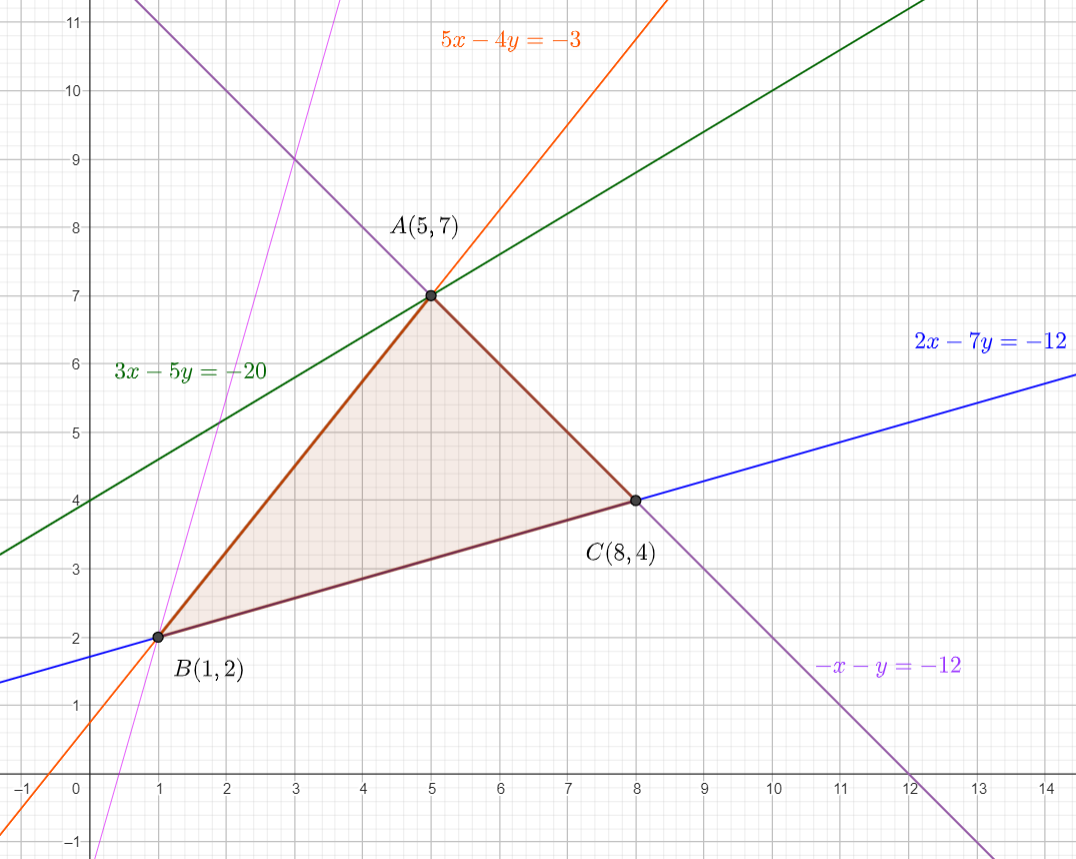
\includegraphics[scale=0.4,frame]{Images/vdhinhhoc.png}
\end{figure}
\begin{itemize}
    \item \textbf{Bước 2:} Xác định các điểm cực biên là $A(5,7); B(1,2); C(8,4)$.
\end{itemize}
\begin{itemize}
    \item \textbf{Bước 3:} Thay toạ độ vào hàm mục tiêu: $f_A = 21$; $f_B = 4$; $f_C=48$. Vậy phương án tối ưu duy nhất của bài toán là $(x,y) = (1,2); f_{min}=3$.
\end{itemize}
\paragraph{Nhận xét:}
\begin{itemize}
    \item [$\square$] Ưu điểm
    \begin{itemize}[label=\textbullet]
        \item Thuật toán đơn giản, dễ hiểu và dễ triển khai.
        \item Trong trường hợp bài toán có số biến và ràng buộc nhỏ, phương pháp hình học có thể đạt hiệu suất tốt và tìm ra giải pháp tối ưu trong thời gian ngắn do đó cũng dễ kiểm tra và hình dung.
    \end{itemize}
    \item [$\square$] Nhược điểm
    \begin{itemize}[label=\textbullet]
        \item Không hiệu quả với các bài toán lớn có số biến và ràng buộc lớn.
        \item Với số biến càng lớn, đòi hỏi không gian nhiều chiều khiến cho việc hình dung và vẽ hình trở nên khó khăn.
    \end{itemize}
\end{itemize}
\newpage
\subsubsection{Thuật toán đơn hình - Simplex method}
\paragraph{Thuật toán:}
\begin{flushleft}
    \hspace{0.4cm} Xét bài toán quy hoạch tuyến tính có dạng như sau:
\end{flushleft}
\begin{itemize}
    \item [$(1)$] $f(x) = c_1x_1+c_2x_2+...+c_nx_n \longrightarrow max(min)$
    \item [$(2)$] $a_{i1}x_1+a_{i2}x_2+...+a_{in}x_n=b_i, i=1,2,...,m$ 
    \item [$(3)$] $x_j\geq 0, j=1,2,...,n$
\end{itemize}
\hspace{0.4cm} Để tìm phương án tối ưu $Danzig$ đã đề xuất thuật toán như sau: xuất phát từ một phương án cực biên $x^0$. Kiểm tra xem $x^0$ có phải là lời giải tối ưu hay chưa. Nếu $x_0$ chưa phải là phương án tối ưu thì tìm cách cải tiến nó để được một phương án cực biên khác là $x^1$ tốt hơn $x^0$ theo nghĩa $Z(x^1)$ $<$ $Z(x^0)$ (max thì ngược lại). Quá trình được lặp lại nhiều lần tới khi tìm thấy cực biên tối ưu.\medskip \\
\indent Thuật toán áp dụng cho bài toán mà các biến đều $\geq 0$ và các ràng buộc ở dạng đẳng thức.\medskip \\
\indent Trước hết, ta phải chọn ra phương án cực biên cơ sở (các hệ số của nó chúng tạo thành ma trận đơn vị). Nếu không có sẵn phương án đó, ta dùng phương pháp big M để tạo biến ảo để có ma trận đơn vị.
\begin{table}[tbh!]
    \large
    \begin{tabular}{|w{c}{2cm}|w{c}{2cm}|w{c}{2cm}|w{c}{2cm}|w{c}{2cm}|w{c}{2cm}|w{c}{2cm}|}
    \hline
        Hệ số & Ẩn cơ bản & Phương án & \begin{tabular}[c]{@{}c@{}}$x_1$\\ $c_1$\end{tabular} & \begin{tabular}[c]{@{}c@{}}$x_2$\\ $c_2$\end{tabular} & \begin{tabular}[c]{@{}c@{}}$x_3$\\ $c_3$\end{tabular} & $\lambda_i$\\ \hline
        $c_1$ & $x_1$ & $b_1$ & $a_{11}$ & $a_{12}$ & $a_{13}$ &\\ \hline
        $c_2$ & $x_2$ & $b_2$ & $a_{21}$ & $a_{22}$ & $a_{23}$ &\\ \hline
        & $f_{min}$ & $\sum b_ic_i$ & $\Delta_1$ & $\Delta_2$ & $\Delta_3$& $\Delta_j$ \\ \hline
    \end{tabular}
\end{table}
\begin{itemize}
    \item Trong bài toán QHTT tìm \textbf{$min$}, thuật toán dừng lại khi tất cả các $\Delta \leq 0$. Nếu còn $\Delta > 0$, ta chọn ra số lớn nhất, và trên cột tương ứng, ta chọn phần tử xoay $a_{ij}$ theo tiêu chí: nó là số dương, xét $\lambda_v =  \displaystyle\min_{a_{iv}>0} \displaystyle\frac{b_i}{a_{iv}}$ từ đó tìm $\max\{\Delta_v . \lambda_v|\forall\Delta_v>0\}$
    \item Trong bài toán QHTT tìm \textbf{$max$}, thuật toán dừng lại khi tất cả các $\Delta \geq 0$. Nếu còn $\Delta < 0$, ta chọn ra số âm nhỏ nhất, và trên cột tương ứng, ta chọn phần tử xoay $a_{ij}$ theo tiêu chí: nó là số dương, xét $\lambda_v =  \displaystyle\min_{a_{iv}>0} \displaystyle\frac{b_i}{a_{iv}}$ từ đó tìm $\max\{|\Delta_v| . \lambda_v|\forall\Delta_v<0\}$
\end{itemize}
\hspace{0.4cm} Sau khi chọn được phần tử xoay, ta sẽ có biến cơ bản vào/ra, và bảng đơn hình mới.\medskip \\
Tóm lại, thuật toán gồm các bước:
\begin{itemize}
    \item [$\square$] \textbf{Bước 1:} Xác định Hàm mục tiêu và ràng buộc.
    \item [$\square$] \textbf{Bước 2:} Chuyển đổi Bất đẳng thức thành Phương trình ($\leq,\geq \longrightarrow =$)
    \item [$\square$] \textbf{Bước 3:} Xác định ma trận hệ số $A=$
    $\left[\begin{array}{l}
        \begin{tabular}{c c c}
            $a_{11}$ & $a_{12}$ & $a_{13}$ \\
            $a_{21}$ & $a_{22}$ & $a_{23}$\\
        \end{tabular}
    \end{array}\right]$ và các ẩn cơ bản \medskip \\
    \item [$\square$] \textbf{Bước 4:} Xây dựng Bảng đơn hình hay Bảng Simplex ban đầu.
    \item [$\square$] \textbf{Bước 5:} Xác định các cột mục tiêu.
    \item [$\square$] \textbf{Bước 6:} Tính các tỷ số rời cơ sở $\lambda_v =  \displaystyle\min_{a_{iv}>0} \displaystyle\frac{b_i}{a_{iv}}$
    \item [$\square$] \textbf{Bước 7:} Thực hiện then chốt nhằm loại bỏ biến rời khỏi cơ sở và đưa biến vào cơ sở.
    \begin{equation*}
        \text{Dòng có ẩn đưa vào}= \text{dòng chuẩn} = \frac{\text{dòng chủ yếu}}{\text{hệ số chủ yếu}}
    \end{equation*}
    \begin{flushleft}
        Dòng thứ $i$ = Dòng thứ $i$ (cũ) - $a_{iv}$.dòng chuẩn. ($a_{iv}$: số nằm trên giao của dòng $i$ và cột chủ yếu).
    \end{flushleft}
    \item [$\square$] \textbf{Bước 8:} Lặp lại các bước 5,6,7 trong trường hợp còn giá trị âm trong hàng hàm mục tiêu (hàng cuối cùng) đối với bài toán tìm $max$ và giá trị dương đối với bài toán tìm $min$.
    \item [$\square$] \textbf{Bước 9:} Ghi nhận kết quả với các giá trị.
\end{itemize}
\paragraph{Ví dụ minh hoạ:}
\begin{flushleft}
    \textbf{\underline{Ví dụ 1:}} Tìm giá trị tối đa của hàm $f(x)=40x_1+30x_2$ $(1)$
\end{flushleft}
\begin{equation*}
    \begin{cases}
        x_1 + x_2 \leq 12\text{ }\text{ }(2)\\
        2x_1 + x_2 \leq 16\text{ }\text{ }(3)\\
        x_1 \geq 0, x_2 \geq 0\text{ }\text{ }(4)
    \end{cases}
\end{equation*}
\begin{itemize}
    \item [$\square$] \textbf{Bước 1:} Xác định hàm mục tiêu và ràng buộc
    \begin{itemize}[label=\textbullet]
        \item Bước này chỉ sử dụng cho các bài toán thực tế cần thiết lập hệ phương trình, hệ bất phương trình dựa trên yêu cầu đề bài.
        \item Vì bài toán đã xác định hàm mục tiêu và các ràng buộc nên ta qua bước thứ 2.
    \end{itemize}
    \item [$\square$] \textbf{Bước 2:} Chuyển đổi Bất đẳng thức thành Phương trình.
    \begin{flushleft}
        Có thể thấy có 2 bất phương trình $(2)$ và $(3)$, ta lần lượt cộng biến thêm vào (biến slack) $x_3$ và $x_4$ cho 2 bất phương trình để chuyển về dạng phương trình.
        \begin{equation*}
            \begin{cases}
                x_1 + x_2 +x_3 = 12\text{ }\text{ }(2)\\
                2x_1 + x_2 +x_4 = 16\text{ }\text{ }(3)\\
            \end{cases}
        \end{equation*}
    \end{flushleft}
    \item [$\square$] \textbf{Bước 3:} Xác định ma trận hệ số và các ẩn cơ bản
    \begin{equation*}
        A = \left[\begin{array}{l}
        \begin{tabular}{c c c c}
            1 & 1 & 1 & 0\\
            2 & 1 & 0 & 1\\
        \end{tabular}
    \end{array}\right]
    \end{equation*}
    \begin{flushleft}
            \indent Có chứa đầy đủ 2 vector cột đơn vị $e_1$ (cột 3), $e_2$ (cột 4)\medskip \\
            \indent Do đó bài toán có dạng chuẩn, trong đó:
            \begin{itemize}
                \item Ẩn cơ bản thứ nhất là $x_3$
                \item Ẩn cơ bản thứ hai là $x_4$
            \end{itemize}
        \end{flushleft}
    \item [$\square$] \textbf{Bước 4:} Xây dựng Bảng Simplex ban đầu
    \begin{flushleft}
        \begin{table}[tbh!]
        \large
        \begin{tabular}{|w{c}{1.75cm}|w{c}{2cm}|w{c}{2cm}|w{c}{1.75cm}|w{c}{1.75cm}|w{c}{1.75cm}|w{c}{1.75cm}|w{c}{1cm}|}
            \hline
            Hệ số & Ẩn cơ bản & Phương án & \begin{tabular}[c]{@{}c@{}}$x_1$\\ 40\end{tabular} & \begin{tabular}[c]{@{}c@{}}$x_2$\\ 30\end{tabular} & \begin{tabular}[c]{@{}c@{}}$x_3$\\ 0\end{tabular} & \begin{tabular}[c]{@{}c@{}}$x_4$\\ 0\end{tabular} & $\lambda_i$\\ \hline
            0 & $x_3$ & 12 & 1 & 1 & 1 & 0&\\ \hline
            0 & $x_4$ & 16 & 2 & 1 & 0 & 1&\\ \hline
             & 0 & 0 & -40 & -30 & 0 & 0&$\Delta_j$\\ \hline
        \end{tabular}
        \end{table}
    \end{flushleft}
    \item [$\square$] \textbf{Bước 5:} Xác định cột mục tiêu.
    \begin{flushleft}
        \hspace{0.4cm} Tìm giá trị âm lớn nhất trong hàng hàm mục tiêu (dòng dưới cùng), dễ thấy cột 4 có giá trị -40 là nhỏ nhất nên cột mục tiêu là cột 4\medskip\\
    \end{flushleft}
    \item [$\square$] \textbf{Bước 6:} Tính tỷ số rời cơ sở
    \begin{flushleft}
    \hspace{0.4cm} Ta lấy các giá trị phương án lần lượt ở dòng 1 và 2 chia cho phần tử ở cột chủ yếu hay cột 4 ở dòng 1 và 2 để tìm giá trị $\lambda_i$
        \begin{table}[tbh!]
        \large
        \begin{tabular}{|w{c}{1.75cm}|w{c}{2cm}|w{c}{2cm}|w{c}{1.75cm}|w{c}{1.75cm}|w{c}{1.75cm}|w{c}{1.75cm}|w{c}{1cm}|}
            \hline
            Hệ số & Ẩn cơ bản & Phương án & \begin{tabular}[c]{@{}c@{}}$x_1$\\ 40\end{tabular} & \begin{tabular}[c]{@{}c@{}}$x_2$\\ 30\end{tabular} & \begin{tabular}[c]{@{}c@{}}$x_3$\\ 0\end{tabular} & \begin{tabular}[c]{@{}c@{}}$x_4$\\ 0\end{tabular} & $\lambda_i$\\ \hline
            0 & $x_3$ & \cellcolor[rgb]{.500,  .749, .749}12 & \cellcolor[rgb]{.500,  .749, .749}1 & 1 & 1 & 0&\cellcolor[rgb]{.500,  .749, .749}12\\ \hline
            0 & $x_4$ & \cellcolor[rgb]{.749,  .749, .749}16 & \cellcolor[rgb]{.749,  .749, .749}2 & 1 & 0 & 1& \cellcolor[rgb]{.749,  .749, .749}8\\ \hline
             &  & 0 & -40 & -30 & 0 & 0&$\Delta_j$\\ \hline
        \end{tabular}
        \end{table}\\
        \hspace{0.4cm} Vì $\lambda_2 = 8$ nhỏ nhất nên dòng chủ yếu là dòng 3.\medskip \\
        \hspace{0.4cm} Giao của cột chủ yếu và dòng chủ yếu là hệ số chủ yếu có giá trị là 2.  
        \begin{table}[tbh!]
        \large
        \begin{tabular}{|w{c}{1.75cm}|w{c}{2cm}|w{c}{2cm}|w{c}{1.75cm}|w{c}{1.75cm}|w{c}{1.75cm}|w{c}{1.75cm}|w{c}{1cm}|}
            \hline
            Hệ số & Ẩn cơ bản & Phương án & \begin{tabular}[c]{@{}c@{}}$x_1$\\ 40\end{tabular} & \begin{tabular}[c]{@{}c@{}}$x_2$\\ 30\end{tabular} & \begin{tabular}[c]{@{}c@{}}$x_3$\\ 0\end{tabular} & \begin{tabular}[c]{@{}c@{}}$x_4$\\ 0\end{tabular} & $\lambda_i$\\ \hline
            0 & $x_3$ & 12 & 1 & 1 & 1 & 0&12\\ \hline
            0 & $x_4$ & 16 & \cellcolor[rgb]{.749,  .800, .749}$2^*$ & 1 & 0 & 1& 8\\ \hline
             &  & 0 & -40 & -30 & 0 & 0&$\Delta_j$\\ \hline
        \end{tabular}
        \end{table}\\
    \end{flushleft}
    \item [$\square$] \textbf{Bước 7:} Thực hiện then chốt. Tính bảng 2 theo công thức sau:
    \begin{equation*}
        \text{Dòng có ẩn đưa vào}= \text{dòng chuẩn} = \frac{\text{dòng chủ yếu}}{\text{hệ số chủ yếu}}
    \end{equation*}
    \begin{flushleft}
        Dòng thứ $i$ = Dòng thứ $i$ (cũ) - $a_{iv}$.dòng chuẩn. ($a_{iv}$: số nằm trên giao của dòng $i$ và cột chủ yếu).
    \end{flushleft}
    \begin{flushleft}
        \begin{table}[tbh!]
        \large
        \begin{tabular}{|w{c}{1.75cm}|w{c}{2cm}|w{c}{2cm}|w{c}{1.75cm}|w{c}{1.75cm}|w{c}{1.75cm}|w{c}{1.75cm}|w{c}{1cm}|}
            \hline
            Hệ số & Ẩn cơ bản & Phương án & \begin{tabular}[c]{@{}c@{}}$x_1$\\ 40\end{tabular} & \begin{tabular}[c]{@{}c@{}}$x_2$\\ 30\end{tabular} & \begin{tabular}[c]{@{}c@{}}$x_3$\\ 0\end{tabular} & \begin{tabular}[c]{@{}c@{}}$x_4$\\ 0\end{tabular} & $\lambda_i$\\ \hline
            0 & $x_3$ & 4 & 0 & $1/2$ & 1 & $-1/2$&8\\ \hline
            40 & $x_1$ & 8 & $1^*$ & $1/2$ & 0 & $1/2$&16 \\ \hline
             &  & 320 & 0 & -10 & 0 & 0&$\Delta_j$\\ \hline
        \end{tabular}
        \end{table}
    \end{flushleft}
\end{itemize}
\begin{itemize}
    \item [$\square$] \textbf{Bước 8:} Lặp lại các bước 4,5,6, ta được bảng sau:
    \begin{flushleft}
        \begin{table}[th!]
        \large
        \begin{tabular}{|w{c}{1.75cm}|w{c}{2cm}|w{c}{2cm}|w{c}{1.75cm}|w{c}{1.75cm}|w{c}{1.75cm}|w{c}{1.75cm}|w{c}{1cm}|}
            \hline
            Hệ số & Ẩn cơ bản & Phương án & \begin{tabular}[c]{@{}c@{}}$x_1$\\ 40\end{tabular} & \begin{tabular}[c]{@{}c@{}}$x_2$\\ 30\end{tabular} & \begin{tabular}[c]{@{}c@{}}$x_3$\\ 0\end{tabular} & \begin{tabular}[c]{@{}c@{}}$x_4$\\ 0\end{tabular} & $\lambda_i$\\ \hline
            30 & $x_2$ & 8 & 0 & 1 & 2 & -1&\\ \hline
            40 & $x_1$ & 4 & 1 & 0 & -1 & 1& \\ \hline
             &  & 400 & 0 & 0 & 20 & 10&$\Delta_j$\\ \hline
        \end{tabular}
        \end{table} 
        \hspace{0.4cm} Không còn số âm trong hàng cuối cùng phương pháp đã tìm được phương án tối ưu, quy trình dừng lại.
    \end{flushleft}
\end{itemize}
\begin{itemize}
    \item [$\square$] \textbf{Bước 9:} Ghi nhận kết quả
    \begin{flushleft}
        \hspace{0.4cm} Kết luận cho bài toán phụ: PATƯ: $X^2 =(x_1,x_2,x_3,x_4)=(4,8,0,0)$
        \begin{equation*}
            \text{GTTƯ: }f(X2)=400 \hspace{1cm}
        \end{equation*}
        \hspace{0.4cm} Kết luận cho bài toán gốc: PATƯ: $X^2 =(x_1,x_2)=(4,8)$
        \begin{equation*}
            \text{GTTƯ: }f(X2)=400 \hspace{1cm}
        \end{equation*}
    \end{flushleft}
\end{itemize}
\textbf{\underline{Ví dụ 2:}} Một công ty xây dựng cần phân phối nguồn lực cho ba dự án khác nhau: Dự án X, Y, và Z. Mỗi dự án cần một số lượng nhất định của ba loại nguồn lực: lao động, vật liệu, và máy móc. Công ty có một lượng hạn chế nguồn lực mỗi ngày và muốn phân phối chúng để tối đa hóa lợi nhuận tổng cộng từ ba dự án. Dưới đây là thông tin chi tiết:
\begin{itemize}
    \item Mỗi dự án X, Y, và Z mang lại lợi nhuận lần lượt là 500, 300, và 400 đô la mỗi ngày.
    \item Mỗi dự án cần nguồn lực như sau:
    \begin{itemize}
        \item Dự án X: 2 lao động, 3 vật liệu, 2 máy móc
        \item Dự án Y: 4 lao động, 1 vật liệu, 1 máy móc
        \item Dự án Z: 3 lao động, 2 vật liệu, 3 máy móc
    \end{itemize}
    \item Công ty có tối đa 100 lao động, 90 vật liệu, và 40 máy móc mỗi ngày.
\end{itemize}
\hspace{0.4cm} Hãy lập mô hình toán học của bài toán xác định số ngày làm việc cho từng dự án sao cho không bị động về nguồn lực mà lợi nhuận đạt về cao nhất\medskip \\
\underline{\textit{Lời giải}} Ở ví dụ này, ta sẽ làm nhanh bài toán. 
Gọi $x_1, x_2, x_3$ lần lượt là số ngày làm việc cho dự án X, Y và Z. Ta có các điều kiện $x_1, x_2, x_3 \geq 0$ \medskip \\
\indent Để không bị động về nguồn lực ta có các điều kiện sau:
\begin{equation*}
    \begin{tabular}{c c c c c l}
        $2x_1$ &$+$ & $4x_2$ & $+$ & $3x_3$ &$\leq 100$  \\
        $3x_1$ &$+$ & \text{ }$x_2$   & $+$ & $2x_3$ &$\leq 90$ \\
        $2x_1$ &$+$ & \text{ }$x_2$   & $+$ & $3x_3$ &$\leq 40$ \\
    \end{tabular}
\end{equation*}
\indent Tổng doanh thu theo dự kiến là: $500x_1+300x_2+400x_3$ \medskip \\
\indent Để doanh thu đạt được cao nhất ta có điều kiện
\begin{equation*}
    500x_1+300x_2+400x_3 \longrightarrow max
\end{equation*}
\indent Như vậy, mô hình toán học của bài toán là:
\begin{equation*}
    (1) \text{ }500x_1+300x_2+400x_3 \longrightarrow max\hspace{0.45cm}
\end{equation*}
\begin{equation*} (2) \Bigg\{
    \begin{tabular}{c c c c c l}
        $2x_1$ &$+$ & $4x_2$ & $+$ & $3x_3$ &$\leq 100$  \\
        $3x_1$ &$+$ & \text{ }$x_2$   & $+$ & $2x_3$ &$\leq 90$ \\
        $2x_1$ &$+$ & \text{ }$x_2$   & $+$ & $3x_3$ &$\leq 40$ \\
    \end{tabular}
\end{equation*}
\begin{equation*}
    (3)\text{ }x_1,x_2,x_3 \geq 0 \hspace{3.8cm}
\end{equation*}
\indent Đưa bài toán về dạng chính tắc ta thêm các ẩn phụ $x_4, x_5, x_6 \geq 0$ sao cho:
\begin{equation*}
    \begin{tabular}{c c c c c c c l}
        $2x_1$ &$+$ &          $4x_2$ & $+$ & $3x_3$ &$+$ & $x_4$ &$= 100$  \\
        $3x_1$ &$+$ & \text{ }$x_2$   & $+$ & $2x_3$ &$+$ & $x_5$ &$= \text{ }90$ \\
        $2x_1$ &$+$ & \text{ }$x_2$   & $+$ & $3x_3$ &$+$ & $x_6$ &$= \text{ }40$ \\
    \end{tabular}
\end{equation*}
\indent Ma trận hệ số của ràng buộc:
$A =\left[\begin{array}{l}
\begin{tabular}{c c c c c c}
    2 & 4 & 3 & 1 & 0 & 0 \\
    3 & 1 & 2 & 0 & 1 & 0 \\
    2 & 1 & 3 & 0 & 0 & 1 \\
\end{tabular}
\end{array}\right]$ \\
\indent Trong đó:
\begin{itemize}
    \item Ẩn cơ bản (1): $x_4=100$
    \item Ẩn cơ bản (2): $x_5=90$
    \item Ẩn cơ bản (3): $x_6=40$
\end{itemize}
\hspace{0.4cm} Ta có phương án xuất phát: $x=(x_1,x_2,x_3,x_4,x_5,x_6)=(0,0,0,100,90,40)$ \medskip \\
\indent Ta xây dựng được bảng Simplex đầu tiên:
\begin{table}[tbh!]
\large
\begin{tabular}{|c|c|c|w{c}{1.15cm}|w{c}{1.15cm}|w{c}{1.15cm}|w{c}{1.15cm}|w{c}{1.15cm}|w{c}{1.15cm}|w{c}{1.15cm}|} \hline
Hệ số & Ẩn cơ bản & Phương án & \begin{tabular}[c]{@{}c@{}}$x_1$\\ 500\end{tabular}   & \begin{tabular}[c]{@{}c@{}}$x_2$\\ 300\end{tabular}   & \begin{tabular}[c]{@{}c@{}}$x_3$\\ 400\end{tabular}   & \begin{tabular}[c]{@{}c@{}}$x_4$\\ 0\end{tabular} & \begin{tabular}[c]{@{}c@{}}$x_5$\\ 0\end{tabular} & \begin{tabular}[c]{@{}c@{}}$x_6$\\ 0\end{tabular} &  $\lambda_i$  \\ \hline
0     & $x_4$        & 100       & 2    & 4    & 3    & 1  & 0  & 0  & 50 \\ \hline
0     & $x_5$        & 90        & 3    & 1    & 2    & 0  & 1  & 0  & 30 \\ \hline
0     & $x_6$        & 40        & 2    & 1    & 3    & 0  & 0  & 1  & 20 \\ \hline
      &           & 0         & -500 & -300 & -400 & 0  & 0  & 0  & $\Delta_j$ \\ \hline
\end{tabular}
\end{table}

\indent Vì $\Delta_j \leq 0$ nên ta tiến hành tạo bảng thứ 2.
\begin{flushleft}
    \hspace{0.4cm} Ta lập được bảng sau:
\end{flushleft} 
\begin{table}[h!]
\large
\begin{tabular}{|c|c|c|w{c}{1.15cm}|w{c}{1.15cm}|w{c}{1.15cm}|w{c}{1.15cm}|w{c}{1.15cm}|w{c}{1.15cm}|w{c}{1.15cm}|}\hline
Hệ số & Ẩn cơ bản & Phương án & \begin{tabular}[c]{@{}c@{}}$x_1$\\ 500\end{tabular}   & \begin{tabular}[c]{@{}c@{}}$x_2$\\ 300\end{tabular}   & \begin{tabular}[c]{@{}c@{}}$x_3$\\ 400\end{tabular}   & \begin{tabular}[c]{@{}c@{}}$x_4$\\ 0\end{tabular} & \begin{tabular}[c]{@{}c@{}}$x_5$\\ 0\end{tabular} & \begin{tabular}[c]{@{}c@{}}$x_6$\\ 0\end{tabular} &  $\lambda_i$  \\ \hline
0     & $x_4$        & 60        & 0  & 3    & 0    & 1  & 0  & -1   & 20                               \\ \hline
0     & $x_5$        & 30        & 0  & $-1/2$ & $-5/2$ & 0  & 1  & $-3/2$ & \textbackslash{}\textbackslash{} \\ \hline
500   & $x_1$        & 20        & 1  & $1/2$  & $3/2$  & 0  & 0  & $1/2$  & 40                               \\ \hline
      &           & 10000      & 0  & -50  & 350  & 0  & 0  & 250  &   $\Delta_j$                               \\ \hline
\end{tabular}
\begin{flushleft}
    \hspace{0.4cm} Vì $\Delta_j \leq 0$ nên ta tiếp tục chuyển sang bảng số 3
\end{flushleft}
\end{table}  
\begin{table}[tbh!]
\large
\begin{tabular}{|c|c|c|w{c}{1.15cm}|w{c}{1.15cm}|w{c}{1.15cm}|w{c}{1.15cm}|w{c}{1.15cm}|w{c}{1.15cm}|w{c}{1.15cm}|} \hline
Hệ số & Ẩn cơ bản & Phương án & \begin{tabular}[c]{@{}c@{}}$x_1$\\ 500\end{tabular}   & \begin{tabular}[c]{@{}c@{}}$x_2$\\ 300\end{tabular}   & \begin{tabular}[c]{@{}c@{}}$x_3$\\ 400\end{tabular}   & \begin{tabular}[c]{@{}c@{}}$x_4$\\ 0\end{tabular} & \begin{tabular}[c]{@{}c@{}}$x_5$\\ 0\end{tabular} & \begin{tabular}[c]{@{}c@{}}$x_6$\\ 0\end{tabular} &  $\lambda_i$  \\ \hline
300   & $x_2$      & 20        & 0  & 1  & 0      & $1/3$  & 0  & $-1/3$  &                                           \\ \hline
0     & $x_5$      & 40        & 0  & 0  & $-5/2$ & $1/6$  & 1  & $-5/3$  &                                           \\ \hline
500   & $x_1$      & 10        & 1  & 0  & $3/2$  & $-1/6$ & 0  & $2/3$   &                                           \\ \hline
      &           & 11000     & 0  & 0  & 350    & $50/3$ & 0  & $700/3$ & $\Delta_j \geq 0$ \\ \hline
\end{tabular}
\end{table} 
\hspace{0.4cm} Kết luận cho bài toán phụ: PATƯ: $X^2 =(x_1,x_2,x_3,x_4,x_5,x_6)=(10,20,0,0,40,0)$
\begin{equation*}
    \text{GTTƯ: }f(X2)=11000 \hspace{1.8cm}
\end{equation*}
\hspace{0.4cm} Kết luận cho bài toán gốc: PATƯ: $X^2 =(x_1,x_2,x_3)=(10,20,0)$
\begin{equation*}
    \text{GTTƯ: }f(X2)=11000 \hspace{1.8cm}
\end{equation*}
\hspace{0.4cm} Vậy để lợi nhuận đạt cao nhất: 
\begin{itemize}
    \item Số ngày làm việc cho dự án X: 20 ngày
    \item Số ngày làm việc cho dự án Y: 10 ngày
    \item Số ngày làm việc cho dự án  Z: 0 ngày
\end{itemize} 
\paragraph{Nhận xét:}
\begin{itemize}
    \item [$\square$] Ưu điểm
    \begin{itemize}[label=\textbullet]
        \item Phương pháp đơn hình thường hiệu quả với các bài toán có số biến và ràng buộc lớn. 
        \item Phương pháp đơn hình có thể giải quyết các bài toán với rất nhiều ràng buộc phức tạp và hàm mục tiêu không tuyến tính, miễn là chúng có thể được biểu diễn dưới dạng tuyến tính.
        \item Có thể dễ dàng tự động hóa phương pháp đơn hình, điều này có nghĩa là nó có thể được triển khai trong các phần mềm hoặc hệ thống thông tin để giải quyết các bài toán tối ưu.
    \end{itemize}
    \item [$\square$] Nhược điểm
    \begin{itemize}[label=\textbullet]
        \item Trong một số trường hợp, phương pháp đơn hình có thể rơi vào một vòng lặp vô hạn mà không thể tìm ra giải pháp tối ưu.
        \item Trong một số trường hợp, phương pháp đơn hình có thể yêu cầu một số lượng lớn các bước lặp để đạt được giải pháp tối ưu, đặc biệt là trên các bài toán có số lượng biến và ràng buộc lớn.
    \end{itemize}
\end{itemize}
\subsubsection{Phương pháp đối ngẫu:}
\paragraph{Thuật toán:}
\begin{flushleft}
    \hspace{0.4cm} Quy tắc chuyển đổi giữa bài toán $min - max$
\end{flushleft}
\begin{itemize}
    \item [$\square$] \textbf{\underline{TH1:}} Bài toán gốc tìm $min$, bài toán đối ngẫu tìm $max$
    \begin{table}[!ht]
        \centering
        \begin{tabular}{|w{c}{6cm}|w{c}{6cm}|}
        \hline
            Bài toán gốc $(P)$ & Bài toán đối ngẫu $(D)$ \\ \hline
            Hệ số hàm mục tiêu & Vế phải của ràng buộc chính \\ \hline
            Ràng buộc chính thứ $i$ dấu $\left(\begin{array}{l} \geq \\ \leq \\= \\ \end{array}\right)$ & Biến thứ $i$ dấu $\left(\begin{array}{l} \geq 0 \\ \leq 0 \\ \text{tuỳ ý} \\ \end{array}\right)$ \\ \hline
            Biến thứ $j$ dấu $\left(\begin{array}{l} \geq 0 \\ \leq 0 \\ \text{tuỳ ý} \\ \end{array}\right)$ & Ràng buộc chính thứ $j$ dấu $\left(\begin{array}{l} \leq \\ \geq \\= \\ \end{array}\right)$ \\ \hline
        \end{tabular}
    \end{table}
    \item [$\square$] \textbf{\underline{TH2:}} Bài toán gốc tìm $max$, bài toán đối ngẫu tìm $min$
    \begin{table}[!ht]
        \centering
        \begin{tabular}{|w{c}{6cm}|w{c}{6cm}|}
        \hline
            Bài toán gốc $(P)$ & Bài toán đối ngẫu $(D)$ \\ \hline
            Hệ số hàm mục tiêu & Vế phải của ràng buộc chính \\ \hline
            Ràng buộc chính thứ $i$ dấu $\left(\begin{array}{l} \geq \\ \leq \\= \\ \end{array}\right)$ & Biến thứ $i$ dấu $\left(\begin{array}{l} \leq 0 \\ \geq 0 \\ \text{tuỳ ý} \\ \end{array}\right)$ \\ \hline
            Biến thứ $j$ dấu $\left(\begin{array}{l} \geq 0 \\ \leq 0 \\ \text{tuỳ ý} \\ \end{array}\right)$ & Ràng buộc chính thứ $j$ dấu $\left(\begin{array}{l} \geq \\ \leq \\= \\ \end{array}\right)$ \\ \hline
        \end{tabular}
    \end{table}
    \item [$\square$] Bài toán đối ngẫu $(D)$ giúp ta khảo sát tính chất của bài toán gốc $(P)$ (mà không đi giải trực tiếp bài gốc), cụ thể là:
    \begin{itemize}[label=\textbullet]
        \item Nếu $(P)$ tìm $max$ thì mỗi phương án của bài $(D)$ sẽ cho ta chặn trên của $(P)$.
        \item Nếu $(P)$ tìm $min$ thì mỗi phương án của bài $(D)$ sẽ cho ta chặn dưới của $(P)$.
    \end{itemize}
    \item [$\square$] Sau khi chuyển thành bài toán đối ngẫu, ta có thể dùng phương pháp đơn hình để tìm phương án tối ưu.
    \item [$\square$] Đối với cặp bài toán đối ngẫu $(P)$ và $(D)$ chỉ xảy ra một trong ba trường hợp sau:
    \begin{itemize}[label=\textbullet]
        \item Cả hai bài toán đều không có phương án tối ưu
        \item Cả hai bài toán đều có phương án, lúc đó chúng đều có phương án tối ưu và giá trị hàm mục tiêu đối với hai phương án tối ưu là bằng nhau.
        \item Một trong hai bài toán không có phương án, còn bài toán kia thì có phương án, khi đó bài toán có phương án không có phương án tối ưu.
    \end{itemize}
\end{itemize}
\paragraph{Ví dụ minh hoạ:}
\begin{flushleft}
    \textbf{\underline{Ví dụ:}} Lập bài toán đối ngẫu của bài toán QHTT sau:
\end{flushleft}
\begin{equation*}
    (P):f(x) = 3x_1+2x_2+1x_3 \longrightarrow max
\end{equation*}
\begin{equation*} \Bigg\{
    \begin{tabular}{c c c c c l}
        $x_1$ &$+$ & $2x_2$ & $-$ & $x_3$ &$\leq 4$  \\
        $2x_1$ &$-$ & \text{ }$x_2$   & $+$ & $x_3$ &$= 8$ \\
        $x_1$ &$-$ & \text{ }$x_2$   &  &  &$\leq 6$ \\
    \end{tabular}
\end{equation*}
\begin{equation*}
    \text{ }x_1,x_2 \geq 0 ; x_3 \text{ tuỳ ý}\hspace{2cm}
\end{equation*}
\hspace{0.4cm} Áp dụng quy tắc chuyển đổi bài toán, ta có:
\begin{equation*}
    (D):f(x) = 4y_1+8y_2+6y_3 \longrightarrow min
\end{equation*}
\begin{equation*} \Bigg\{
    \begin{tabular}{c c c c c l}
        $y_1$ &$+$ & $2y_2$ & $+$ & $y_3$ &$\geq 3$  \\
        $2y_1$ &$-$ & \text{ }$y_2$   & $-$ & $y_3$ &$\geq 2$ \\
        $-$$y_1$ &$+$ & \text{ }$y_2$   &  &  &$= 6$ \\
    \end{tabular}
\end{equation*}
\begin{equation*}
    \text{ }y_1 \geq 0 ; y_2 \text{ tuỳ ý}; y_3 \geq 0\hspace{1.3cm}
\end{equation*}
\paragraph{Nhận xét:}
\begin{itemize}
    \item [$\square$] Ưu điểm:
    \begin{itemize}
        \item Phương pháp đối ngẫu đưa ta một góc nhìn khác để giải bài toán, đôi khi việc giải bài toán gốc tốn nhiều công sức hơn bài toán đối ngẫu.
        \item Phương pháp đối ngẫu sẽ là một công cụ mạnh khi kết hợp với thuật toán đơn hình.
    \end{itemize}
    \item [$\square$] Nhược điểm:
    \begin{itemize}
        \item Trong một vài trường hợp, bài toán đối ngẫu sẽ phức tạp hơn bài toán gốc.
        \item Phương pháp đối ngẫu có thể bị mắc kẹt ở một giải pháp không tối ưu và không thể tìm thấy giải pháp tốt hơn.
    \end{itemize}
\end{itemize}
\newpage
\phantomsection
\section*{III. PHẦN MỀM TÌM PHƯƠNG ÁN TỐI ƯU CHO BÀI TOÁN VẬN TẢI}
\addcontentsline{toc}{section}{\protect\numberline{}III. PHẦN MỀM TÌM PHƯƠNG ÁN TỐI ƯU CHO BÀI TOÁN VẬN TẢI}
\setcounter{section}{1}\setlength{\baselineskip}{15pt}
   % đếm số cho section2, nếu không là hiện 0.1, 0.1.1
\setcounter{subsection}{0}
\setcounter{subsubsection}{0}
\setcounter{paragraph}{0}
\subsection{Bài toán vận tải:}
\hspace{0.4cm} Ta có mô hình bài toán vận tải như sau:
\begin{equation*}
        \min{f(x)} = \sum_{i=1}^m \sum_{j=1}^n c_{ij}x_{ij} \text{ }\text{ }\text{ }\text{ }
\end{equation*}
\begin{equation*}
    \begin{cases}
        \displaystyle \sum_{j=1}^n x_{ij} = s_i \text{ với } (i=1,...,m) \\
        \displaystyle \sum_{i=1}^m x_{ij} = d_j \text{ với } (j=1,...,n) \\
        \displaystyle x_{ij} \geq 0,(i=1,...,m); (j=1,...,n) \\
    \end{cases}
\end{equation*}
\begin{itemize}
    \item [$\square$] Trong đó:
    \begin{itemize}[label=\textbullet]
        \item $m$: Tổng số điểm cung cấp (điểm nguồn).
        \item $n$: Tổng số điểm tiêu thụ (điểm đích).
        \item $s_i$: Khả năng cung cấp của điểm nguồn thứ $i$ $i=(1,2,...,m)$.
        \item $d_j$: Nhu cầu tiêu thụ của điểm đích thứ $j$ $j=(1,2,...,n)$.
        \item $c_{ij}$: Cước phí vận chuyển từ điểm nguồn $i$ tới điểm đích $j$.
        \item $x_{ij}$: Lượng hàng được vận chuyển từ điểm nguồn $i$ tới điểm đích $j$.
    \end{itemize}
\end{itemize}
\hspace{0.4cm} Ta có tổng số hàng dự trữ ở $m$ điểm phát (cung) là $\sum_{j=1}^n s_i$\medskip \\
\indent Và tổng số nhu cầu của n điểm thu (cầu)là $\sum_{i=1}^m d_j$\medskip \\
\indent Cân bằng cung cầu:
\begin{itemize}
    \item [$\square$] Nếu $\sum_{j=1}^n s_i = \sum_{i=1}^m d_j$ thì ta nói bài toán cân bằng thu phát, do đó có thể dùng phương án cực biên để tìm cước phí nhỏ nhất.
    \item [$\square$] Ngược lại, bài toán không cân bằng thu phát khi:
    \begin{itemize}[label=\textbullet]
        \item \underline{TH1:} Cung nhiều hơn cầu: $\sum_{j=1}^n s_i > \sum_{i=1}^m d_j$ thì một số hàng hoá được để lại ở các điểm phát. Ta biểu diễn việc này bằng cách bổ sung một điểm thu giả $d_{n+1}$ với cước phí $c_{i,n+1}=0$ với mọi $i=1,...,n$.
        \item \underline{TH2:} Cung ít hơn cầu: $\sum_{j=1}^n s_i < \sum_{i=1}^m d_j$ thì một số hàng hóa sẽ thiếu cho các điểm thu. Ta biểu diễn việc này bằng cách bổ sung một điểm phát giả $s_{m+1}$ với cước phí $c_{m+1,j}=0$ với mọi $j=1,...,m$. 
    \end{itemize}
    \item [$\square$] Do đó, \textbf{bài toán vận tải luôn có thể đưa về dạng cân bằng thu phát.}
\end{itemize}
\begin{table}[ht]
\large
\begin{center}
\begin{tabular}{|l|w{c}{1.5cm}|w{c}{1.5cm}|w{c}{1.5cm}|w{c}{1.5cm}|l|} \hline
    Kho $(i)$ & \multicolumn{4}{c|}{Điểm bán lẻ $(j)$} & Tổng cung \\ \cline{2-5}
              & 1    & 2   & ...   & m    & \\ \hline 
    1         & $\text{\hspace{1.2cm}}^{c_{11}}$ &$\text{\hspace{1.2cm}}^{c_{12}}$ & ...   & $\text{\hspace{1.2cm}}^{c_{1m}}$ & $s_1$ \\  
              &   &     &       &      & \\ \hline
    2         & $\text{\hspace{1.2cm}}^{c_{21}}$ &$\text{\hspace{1.2cm}}^{c_{22}}$ & ...   & $\text{\hspace{1.2cm}}^{c_{2m}}$ & $s_2$ \\ 
              &      &     &       &      & \\ \hline
    ...       & ...  &...  & ...   & ...  & ... \\ 
              &      &     &       &      & \\ \hline
    n         & $\text{\hspace{1.2cm}}^{c_{n1}}$ &$\text{\hspace{1.2cm}}^{c_{n2}}$ & ...   & $\text{\hspace{1.2cm}}^{c_{nm}}$ & $s_n$ \\ 
              &      &     &       &      & \\ \hline
    Tổng cầu  &$d_1$ &$d_2$& ...   & $d_m$ & $\sum_{j=1}^n s_i \text{ hoặc } \sum_{i=1}^m d_j$\\ \hline
\end{tabular}
\end{center}
\end{table}
\begin{itemize}
     \item [$\square$] Tiêu chí chung để chọn lượng hàng và loại cột/hàng:
        \begin{equation*}
            x_{ij}=min\{s_i; d_j\} = \begin{cases}
                s_i \hspace{2cm} \text{ loại dòng } i, d_j=d_j-s_i \\
                d_j \hspace{2cm} \text{ loại cột } j, s_i=s_i-d_j \\
                s_i = d_j \hspace{1.13cm}  \text{ loại dòng $i$ cột $j$}
            \end{cases}
        \end{equation*}
\end{itemize}
\subsubsection{Phương án cực biên cơ bản:}
\begin{itemize}
    \item [$\square$] Phương án cực biên không suy biến
    \begin{itemize}[label=\textbullet]
        \item Số ô được chọn bằng $m+n-1$.
    \end{itemize}
    \item [$\square$] Phương án cực biên suy biến
    \begin{itemize}[label=\textbullet]
        \item Số ô được chọn nhỏ hơn $m+n-1$.
        \item Ta sẽ chọn thêm một ô có giá trị nhỏ nhất theo thứ từ trên xuống, trái sang phải và không tạo thành chu trình.
    \end{itemize}
\end{itemize}
\subsubsection{Phương pháp Tây Bắc:}
\begin{itemize}
    \item [$\square$] Phương án dễ thực hiện nhưng kém hiệu quả:
    \begin{itemize}[label=\textbullet]
        \item Chọn ô ở góc trái trên cùng (hay góc Tây Bắc) làm nơi xuất phát.
        \item Cung cấp tối đa từ khả năng của điểm nguồn cho các điểm đích theo thứ tự từ trái sang phải. Nếu nguồn $i$ đã hết thì chuyển sang nguồn $i+1$.
        \item Đáp ứng tối đa nhu cầu của 1 điểm đích tới các nguồn theo thứ tự ưu tiên từ trên xuống dưới. Nhu cầu $j$ đã đủ thì chuyển sang như cầu $j+1$.
    \end{itemize}
    \item [$\square$] \textbf{\underline{VD:}} Giả sử ta có bài toán cân bằng thu phát sau:
\end{itemize}
\begin{table}[ht]
\large
\begin{center}
\begin{tabular}{|l|w{c}{1.5cm}|w{c}{1.5cm}|w{c}{1.5cm}|w{c}{1.5cm}|l|} \hline
    Kho $(i)$ & \multicolumn{4}{c|}{Điểm bán lẻ $(j)$} & Tổng cung \\ \cline{2-5}
              & 1    & 2   & 3   & 4    & \\ \hline 
    1         & \cellcolor[rgb]{.749,  .749, .600}$\text{\hspace{1.2cm}}^{c_{11}}$ &\cellcolor[rgb]{.749,  .749, .4}$\text{\hspace{1.2cm}}^{c_{12}}$ & $\text{\hspace{1.2cm}}^{c_{13}}$ & $\text{\hspace{1.2cm}}^{c_{14}}$ & 190 \\  
              &  \cellcolor[rgb]{.749,  .749, .600} 90 & \cellcolor[rgb]{.749,  .749, .400}100 &       &      & \\ \hline
    2         & $\text{\hspace{1.2cm}}^{c_{21}}$ &\cellcolor[rgb]{.749,  .749, .3}$\text{\hspace{1.2cm}}^{c_{22}}$ &\cellcolor[rgb]{.749,  .749, .2}$\text{\hspace{1.2cm}}^{c_{23}}$    & $\text{\hspace{1.2cm}}^{c_{24}}$ & 140 \\ 
              &      & \cellcolor[rgb]{.749,  .749, .300}50  &  \cellcolor[rgb]{.749,  .749, .200}90  &      & \\ \hline
    3       & $\text{\hspace{1.2cm}}^{c_{31}}$ &$\text{\hspace{1.2cm}}^{c_{32}}$ &   \cellcolor[rgb]{.8,  .8, .2}$\text{\hspace{1.2cm}}^{c_{33}}$ & $\text{\hspace{1.2cm}}^{c_{34}}$ &  \\ 
              &      &     & \cellcolor[rgb]{.8,  .8, .2}170 &      &170 \\ \hline
    4         & $\text{\hspace{1.2cm}}^{c_{41}}$ &$\text{\hspace{1.2cm}}^{c_{42}}$ &  $\text{\hspace{1.2cm}}^{c_{43}}$\cellcolor[rgb]{.9,  .9, .2}  & \cellcolor[rgb]{.999,  .999, .1}$\text{\hspace{1.2cm}}^{c_{44}}$ &  \\ 
              &      &     & \cellcolor[rgb]{.9,  .9, .2}40    & \cellcolor[rgb]{.999,  .999, .1}210 &250 \\ \hline
    Tổng cầu  &90 &150& 300   &  210 & 750\\ \hline
\end{tabular}
\end{center}
\end{table}
\begin{itemize}
    \item [$\square$] Giải thích:
    \begin{itemize}[label=\textbullet]
        \item Đầu tiên, chọn ô $(i,j)=(1,1)$ do nguồn cung là $s_1=190 > 90= d_1$ nên $x_{11} = 90$ và loại cột $j = 1$ theo tiêu chí chung. Khi này nguồn cung $s_1' = s_1 - d_1 = 100$.
        \item Vì cột $j=1$ đã bỏ, nên ta xét ô $(i,j)=(1,2)$ và do $s_1' = 100 < d_2$ nên $x_{12} = 100$. Khi nào nhu cầu $d_2'=d_2-s_1'=50$.
        \item Tiếp tục làm như vậy, ta được bảng trên.
    \end{itemize}
\end{itemize}
\subsubsection{Phương pháp cước phí nhỏ nhất:}
\begin{itemize}
    \item [$\square$] Phương án hiệu quả hơn phương pháp Tây Bắc:
    \begin{itemize}[label=\textbullet]
        \item Ưu tiên chọn ô có cước phí nhỏ nhất từ trên xuống dưới để đáp ứng tối đa khả năng cũng như nhu cầu.
        \item Tiến hành bỏ qua những ô của điểm nguồn (bỏ hàng nhu cầu) hoặc điểm đích (bỏ cột cung cấp) đã hết khả năng cung cấp cũng như nhu cầu.
        \item Xác định lại ô có chi phí thấp nhất trong các ô còn lại và tiếp tục phân bổ giống như các bước trên.
    \end{itemize}
    \item [$\square$] \textbf{\underline{VD:}} Giả sử ta có bài toán cân bằng thu phát sau:
\end{itemize}
\begin{table}[ht]
\large
\begin{center}
\begin{tabular}{|l|w{c}{1.5cm}|w{c}{1.5cm}|w{c}{1.5cm}|w{c}{1.5cm}|l|} \hline
    Kho $(i)$ & \multicolumn{4}{c|}{Điểm bán lẻ $(j)$} & Tổng cung \\ \cline{2-5}
              & 1    & 2   & 3   & 4    & \\ \hline 
    1         & $\text{\hspace{1.2cm}}^{4}$ & \cellcolor[rgb]{.749,  .749, .600}$\text{\hspace{1.2cm}}^{1}$ & $\text{\hspace{1.2cm}}^{7}$ & $\text{\hspace{1.2cm}}^{4}$ & 190 \\  
              &$\boxed{}$  &\cellcolor[rgb]{.749,  .749, .600}150& $\boxed{}$&   40 & \\ \hline
    2         & $\text{\hspace{1.2cm}}^{6}$ & $\text{\hspace{1.2cm}}^{8}$ & \cellcolor[rgb]{.9,  .9, .100}$\text{\hspace{1.2cm}}^{3}$ & $\text{\hspace{1.2cm}}^{5}$ & 140 \\ 
              &$\boxed{}$  &   $\boxed{}$& \cellcolor[rgb]{.9,  .9, .100}50 & 90 & \\ \hline
    3       &  \cellcolor[rgb]{.749,  .749, .200}$\text{\hspace{1.2cm}}^{3}$ &$\text{\hspace{1.2cm}}^{9}$ &   $\text{\hspace{1.2cm}}^{11}$ & $\text{\hspace{1.2cm}}^{10}$ &  \\ 
              & \cellcolor[rgb]{.749,  .749, .200}90 &   $\boxed{}$&$\boxed{}$ &80   &170 \\ \hline
    4         & $\text{\hspace{1.2cm}}^{8}$ &$\text{\hspace{1.2cm}}^{6}$ &  \cellcolor[rgb]{.749,  .749, .400}$\text{\hspace{1.2cm}}^{2}$  & $\text{\hspace{1.2cm}}^{12}$ &  \\ 
              & $\boxed{}$ &   $\boxed{}$&\cellcolor[rgb]{.749,  .749, .400}250& $\boxed{}$ &250 \\ \hline
    Tổng cầu  &90 &150& 300   &  210 & 750\\ \hline
\end{tabular}
\end{center}
\end{table}
\begin{itemize}
    \item [$\square$] Giải thích:
    \begin{itemize}[label=\textbullet]
        \item Đầu tiên, chọn ô $(i,j)=(1,2)$ do có cước phí nhỏ nhất với $c_{12}=1$, vì $s_1= 190>150=d_2$ nên $x_{12} = 150$, tiến hành loại bỏ cột 2.
        \item Lặp lại việc tìm kiếm, chọn ô $(4,3)$ với $c_{43}=2$, ta có $x_{43}=250$ loại bỏ hàng 4.
        \item Tiếp tục làm như vậy, ta được bảng trên.
    \end{itemize}
\end{itemize}
\subsubsection{Thuật toán thế vị:}
Thuật toán thế vị chính là thuật toán đơn hình cho bài toán vận tải
\begin{itemize}
    \item [$\square$] \textbf{Bước 1:} Xác định các thế vị $u_i,i=1,...,n$ và $v_j,j=1,...,m$ tương ứng với phương án cực biên $x_0$ bằng việc giải hệ phương trình:
    \begin{equation*}
        u_i+v_j=c_{ij}\text{ } \forall i,j
    \end{equation*}
    \item [$\square$] \textbf{Bước 2:} Tính các ước lượng $\Delta_{ij} = u_i + v_j - c_{ij}$
    \item [$\square$] \textbf{Bước 3:} Nếu $\Delta_{ij} \leq 0$ với mọi $(i=1,...,m)$ và $(j=1,...,n)$. Thuật toán dừng lại, ta có phương án tối ưu. Nếu không, chuyển sang \textit{bước 4}.
    \item [$\square$] \textbf{Bước 4:} 
    \begin{itemize}
        \item [1.] Xác định ô điều chỉnh $(i_s,j_s)$ với 
        \begin{equation*}
            \Delta_{i_s,j_s} = max\{\Delta_{ij}>0|(i=1,...,m);(j=1,...,n)\}
        \end{equation*}
        \item [2.] Xét chu trình chứa ô đó và các ô chọn ban đầu
        \item [3.] Đánh dấu $+/-$ xen kẽ vào chu trình này. Với dấu $+$ được đánh cho ô chọn.
        \item [4.] Xác định $x_{ij}$ nhỏ nhất trong các ô được gán dấu $(-)$.
        \item [5.] Bớt đi một lượng $x_{ij}$ ở các ô được gán dấu $(-)$ và thêm một lượng $x_{ij}$ ở các ô được gán dấu $(+)$. Quay lại \textit{bước 2}.
    \end{itemize}
    \item [$\square$] \textbf{Chú ý:} Cần thành lập phương án cực biên ban đầu (xuất phát) theo Nguyên lý phân bố tối đa với các ô chọn phân bổ bằng các phương pháp: góc Tây Bắc, cước phí thấp nhất,...
\begin{table}[ht]
\large
\begin{center}
\begin{tabular}{|l|w{c}{1.5cm}|w{c}{1.5cm}|w{c}{1.5cm}|w{c}{1.5cm}|l|w{c}{1.5cm}|} \hline
    Kho $(i)$ & \multicolumn{4}{c|}{Điểm bán lẻ $(j)$} & Tổng cung & \\ \cline{2-5}
              & 1    & 2   & ...   & m    & & $u_i$\\ \hline 
    1         & $\text{\hspace{1.2cm}}^{c_{11}}$ &$\text{\hspace{1.2cm}}^{c_{12}}$ & ...   & $\text{\hspace{1.2cm}}^{c_{1m}}$ & $s_1$ & \\  
              &   &     &       &      &  & $u_1$\\ \hline
    2         & $\text{\hspace{1.2cm}}^{c_{21}}$ &$\text{\hspace{1.2cm}}^{c_{22}}$ & ...   & $\text{\hspace{1.2cm}}^{c_{2m}}$ & $s_2$  &\\ 
              &      &     &       &      &  &$u_2$\\ \hline
    ...       & ...  &...  & ...   & ...  & ...  &...\\ 
              &      &     &       &      &  &\\ \hline
    n         & $\text{\hspace{1.2cm}}^{c_{n1}}$ &$\text{\hspace{1.2cm}}^{c_{n2}}$ & ...   & $\text{\hspace{1.2cm}}^{c_{nm}}$ & $s_n$  &\\ 
              &      &     &       &      &  &$u_n$\\ \hline
    Tổng cầu  &$d_1$ &$d_2$& ...   & $d_m$ & $\sum_{j=1}^n s_i \text{ hoặc } \sum_{i=1}^m d_j$ &\\ \hline
    $v_j$ & $v_1$ & $v_2$& ... & $v_m$& &  \\ \hline 
\end{tabular}
\end{center}
\end{table}
    \item [$\square$] \textbf{\underline{Ví dụ 1.4:}} Ta có bảng của bài toán vận tải như sau. Hãy tìm phương án tối ưu. \label{fig:VD}
\begin{table}[ht]
\large
\begin{center}
\begin{tabular}{|l|w{c}{1.5cm}|w{c}{1.5cm}|w{c}{1.5cm}|w{c}{1.5cm}|l|w{c}{1.5cm}|} \hline
    Kho $(i)$ & \multicolumn{4}{c|}{Điểm bán lẻ $(j)$} & Tổng cung & \\ \cline{2-5}
              & 1    & 2   & 3   & 4    & & $u_i$\\ \hline 
    1         & $\text{\hspace{1.2cm}}^{1}$ &$\text{\hspace{1.2cm}}^{2}$ & $\text{\hspace{1.2cm}}^{4}$   & $\text{\hspace{1.2cm}}^{3}$ & 60 & \\  
              &   &     &       &      &  & $u_1$\\ \hline
    2         & $\text{\hspace{1.2cm}}^{2}$ &$\text{\hspace{1.2cm}}^{3}$ & $\text{\hspace{1.2cm}}^{2}$   & $\text{\hspace{1.2cm}}^{7}$ & 70  &\\ 
              &      &     &       &      &  &$u_2$\\ \hline
    3         & $\text{\hspace{1.2cm}}^{3}$ &$\text{\hspace{1.2cm}}^{5}$ & $\text{\hspace{1.2cm}}^{6}$   & $\text{\hspace{1.2cm}}^{4}$ & 20  &\\ 
              &      &     &       &      &  &$u_3$\\ \hline
    Tổng cầu  &30 &40& 30   & 50 & $\sum_{j=1}^n s_i \text{ hoặc } \sum_{i=1}^m d_j$ &\\ \hline
    $v_j$ & $v_1$ & $v_2$& $v_3$ & $v_m$& &  \\ \hline 
\end{tabular}
\end{center}
\end{table}
    \begin{itemize}[label=\textbullet]
        \item Dùng phương pháp cước phí nhỏ nhất xác định nghiệm ban đầu của bài toán:
        \begin{table}[ht]
        \large
        \begin{center}
        \begin{tabular}{|l|w{c}{1.5cm}|w{c}{1.5cm}|w{c}{1.5cm}|w{c}{1.5cm}|l|w{c}{1.5cm}|} \hline
            Kho $(i)$ & \multicolumn{4}{c|}{Điểm bán lẻ $(j)$} & Tổng cung & \\ \cline{2-5}
                      & 1    & 2   & 3   & 4    & & $u_i$\\ \hline 
            1         & \cellcolor[rgb]{.749,  .749, .749}$\text{\hspace{1.2cm}}^{1}$ & \cellcolor[rgb]{.749,  .749, .749}$\text{\hspace{1.2cm}}^{2}$ & $\boxed{ }$ $\text{\hspace{1cm}}^{4}$   & $\boxed{ }$$\text{\hspace{1cm}}^{3}$ & 60 & \\  
                      & \cellcolor[rgb]{.749,  .749, .749} 30 & \cellcolor[rgb]{.749,  .749, .749} 30   &      &     &  &$u_1$\\ \hline
            2         & $\boxed{ }$$\text{\hspace{1cm}}^{2}$ & \cellcolor[rgb]{.749,  .749, .749}$\text{\hspace{1.2cm}}^{3}$ & \cellcolor[rgb]{.749,  .749, .749}$\text{\hspace{1.2cm}}^{2}$   & \cellcolor[rgb]{.749,  .749, .749}$\text{\hspace{1.2cm}}^{7}$ & 70  &\\ 
                      &     & \cellcolor[rgb]{.749,  .749, .749} 10  & \cellcolor[rgb]{.749,  .749, .749} 30     & \cellcolor[rgb]{.749,  .749, .749} 30  &  &$u_2$\\ \hline
            3         & $\boxed{ }$$\text{\hspace{1cm}}^{3}$ &$\boxed{ }$$\text{\hspace{1cm}}^{5}$ & $\boxed{ }$$\text{\hspace{1cm}}^{6}$   & \cellcolor[rgb]{.749,  .749, .749}$\text{\hspace{1.2cm}}^{4}$ & 20  &\\ 
                      &     &    &      & \cellcolor[rgb]{.749,  .749, .749} 20  &  &$u_3$\\ \hline
            Tổng cầu  &30 &40& 30   & 50 & $\sum_{j=1}^n s_i \text{ hoặc } \sum_{i=1}^m d_j$ &\\ \hline
            $v_j$ & $v_1$ & $v_2$& $v_3$ & $v_m$& &  \\ \hline 
        \end{tabular}
        \end{center}
        \end{table}
        \item Đây là phương án xuất phát cơ bản không suy biến, do có $m+n-1=4+3-1=6$ ô chọn.
        \item \textbf{Bước 1:} Xác định các thế vị bằng cách giải hệ phương trình
            \begin{itemize}
                \item $u_1 = 0$; $u_1 + v_1 = 1 \longrightarrow v_1=1$
                \item $u_1=0$; $u_1+v_2 = 2\longrightarrow v_2=2$ 
                \item $v_2=2$; $u_2+v_2 = 3\longrightarrow u_2=1$
                \item $u_2 = 1$; $u_2 + v_3 = 2 \longrightarrow v_3 = 1$
                \item $u_2 = 1$; $u_2 + v_4 = 7 \longrightarrow v_3 = 6$
                \item $v_4 = 6$; $u_3 + v_4 = 4 \longrightarrow u_3 = -2$
            \end{itemize}
        \begin{table}[ht]
        \large
        \begin{center}
        \begin{tabular}{|l|w{c}{1.5cm}|w{c}{1.5cm}|w{c}{1.5cm}|w{c}{1.5cm}|l|w{c}{1.5cm}|} \hline
            Kho $(i)$ & \multicolumn{4}{c|}{Điểm bán lẻ $(j)$} & Tổng cung & \\ \cline{2-5}
                      & 1    & 2   & 3   & 4    & & $u_i$\\ \hline 
            1         & \cellcolor[rgb]{.749,  .749, .749}$\text{\hspace{1.2cm}}^{1}$ & \cellcolor[rgb]{.749,  .749, .749}$\text{\hspace{1.2cm}}^{2}$ & $\boxed{ }$ $\text{\hspace{1cm}}^{4}$   & $\boxed{ }$$\text{\hspace{1cm}}^{3}$ & 60 & \\  
                      & \cellcolor[rgb]{.749,  .749, .749} 30 & \cellcolor[rgb]{.749,  .749, .749} 30   &      &     &  &0\\ \hline
            2         & $\boxed{ }$$\text{\hspace{1cm}}^{2}$ & \cellcolor[rgb]{.749,  .749, .749}$\text{\hspace{1.2cm}}^{3}$ & \cellcolor[rgb]{.749,  .749, .749}$\text{\hspace{1.2cm}}^{2}$   & \cellcolor[rgb]{.749,  .749, .749}$\text{\hspace{1.2cm}}^{7}$ & 70  &\\ 
                      &     & \cellcolor[rgb]{.749,  .749, .749} 10  & \cellcolor[rgb]{.749,  .749, .749} 30     & \cellcolor[rgb]{.749,  .749, .749} 30  &  &1\\ \hline
            3         & $\boxed{ }$$\text{\hspace{1cm}}^{3}$ &$\boxed{ }$$\text{\hspace{1cm}}^{5}$ & $\boxed{ }$$\text{\hspace{1cm}}^{6}$   & \cellcolor[rgb]{.749,  .749, .749}$\text{\hspace{1.2cm}}^{4}$ & 20  &\\ 
                      &     &    &      & \cellcolor[rgb]{.749,  .749, .749} 20  &  &-2\\ \hline
            Tổng cầu  &30 &40& 30   & 50 & $\sum_{j=1}^n s_i \text{ hoặc } \sum_{i=1}^m d_j$ &\\ \hline
            $v_j$ & 1 & 2& 1 & 6& &  \\ \hline 
        \end{tabular}
        \end{center}
        \end{table}
        \item \textbf{Bước 2:} Tính các ước lượng
        \begin{table}[ht]
        \large
        \begin{center}
        \begin{tabular}{|l|w{c}{1.5cm}|w{c}{1.5cm}|w{c}{1.5cm}|w{c}{1.5cm}|l|w{c}{1.5cm}|} \hline
            Kho $(i)$ & \multicolumn{4}{c|}{Điểm bán lẻ $(j)$} & Tổng cung & \\ \cline{2-5}
                      & 1    & 2   & 3   & 4    & & $u_i$\\ \hline 
            1         & \cellcolor[rgb]{.749,  .749, .749}$\text{\hspace{1.2cm}}^{1}$ & \cellcolor[rgb]{.749,  .749, .749}$\text{\hspace{1.2cm}}^{2}$ & $\boxed{ }$ $\text{\hspace{1cm}}^{4}$   & $\boxed{ }$$\text{\hspace{1cm}}^{3}$ & 60 & \\  
                      & \cellcolor[rgb]{.749,  .749, .749} 30 & \cellcolor[rgb]{.749,  .749, .749} 30   &  \colorbox{yellow}{-3}    &    \colorbox{yellow}{3}  &  & 0\\ \hline
            2         & $\boxed{ }$$\text{\hspace{1cm}}^{2}$ & \cellcolor[rgb]{.749,  .749, .749}$\text{\hspace{1.2cm}}^{3}$ & \cellcolor[rgb]{.749,  .749, .749}$\text{\hspace{1.2cm}}^{2}$   & \cellcolor[rgb]{.749,  .749, .749}$\text{\hspace{1.2cm}}^{7}$ & 70  &\\ 
                      &   \colorbox{yellow}{0}  & \cellcolor[rgb]{.749,  .749, .749} 10  & \cellcolor[rgb]{.749,  .749, .749} 30     & \cellcolor[rgb]{.749,  .749, .749} 30  &  &1\\ \hline
            3         & $\boxed{ }$$\text{\hspace{1cm}}^{3}$ &$\boxed{ }$$\text{\hspace{1cm}}^{5}$ & $\boxed{ }$$\text{\hspace{1cm}}^{6}$   & \cellcolor[rgb]{.749,  .749, .749}$\text{\hspace{1.2cm}}^{4}$ & 20  &\\ 
                      &    \colorbox{yellow}{-4} & \colorbox{yellow}{-5}   &  \colorbox{yellow}{-7}    & \cellcolor[rgb]{.749,  .749, .749} 20  &  &-2\\ \hline
            Tổng cầu  &30 &40& 30   & 50 & $\sum_{j=1}^n s_i \text{ hoặc } \sum_{i=1}^m d_j$ &\\ \hline
            $v_j$ & 1 & 2& 1 & 6& &  \\ \hline 
        \end{tabular}
        \end{center}
        \end{table}
        \item \textbf{Bước 3:} Vì $\Delta_{14} = 3 > 0$ nên ta chuyển sang \textbf{Bước 4:}.
        \begin{table}[ht]
        \large
        \begin{center}
        \begin{tabular}{|l|w{c}{1.5cm}|w{c}{1.5cm}|w{c}{1.5cm}|w{c}{1.5cm}|l|w{c}{1.5cm}|} \hline
            Kho $(i)$ & \multicolumn{4}{c|}{Điểm bán lẻ $(j)$} & Tổng cung & \\ \cline{2-5}
                      & 1    & 2   & 3   & 4    & & $u_i$\\ \hline 
            1         & \cellcolor[rgb]{.749,  .749, .749}$\text{\hspace{1.2cm}}^{1}$ & $\boxed{ \textbf{---} }$\cellcolor[rgb]{.749,  .749, .749}$\text{\hspace{1.1cm}}^{2}$ & $\boxed{ }$ $\text{\hspace{1cm}}^{4}$   & $\boxed{ \textbf{+} }$$\text{\hspace{0.8cm}}^{3}$ & 60 & \\  
                      & \cellcolor[rgb]{.749,  .749, .749} 30 & \cellcolor[rgb]{.749,  .749, .749} 30   &  \colorbox{yellow}{-3}    &    \colorbox{yellow}{3}  &  & 0\\ \hline
            2         & $\boxed{ }$$\text{\hspace{1cm}}^{2}$ & $\boxed{ \textbf{+} }$\cellcolor[rgb]{.749,  .749, .749}$\text{\hspace{1.1cm}}^{3}$ & \cellcolor[rgb]{.749,  .749, .749}$\text{\hspace{1.2cm}}^{2}$   & $\boxed{ \textbf{---} }$\cellcolor[rgb]{.749,  .749, .749}$\text{\hspace{1.1cm}}^{7}$ & 70  &\\ 
                      &   \colorbox{yellow}{0}  & \cellcolor[rgb]{.749,  .749, .749} 10  & \cellcolor[rgb]{.749,  .749, .749} 30     & \cellcolor[rgb]{.749,  .749, .749} 30  &  &1\\ \hline
            3         & $\boxed{ }$$\text{\hspace{1cm}}^{3}$ &$\boxed{ }$$\text{\hspace{1cm}}^{5}$ & $\boxed{ }$$\text{\hspace{1cm}}^{6}$   & \cellcolor[rgb]{.749,  .749, .749}$\text{\hspace{1.2cm}}^{4}$ & 20  &\\ 
                      &    \colorbox{yellow}{-4} & \colorbox{yellow}{-5}   &  \colorbox{yellow}{-7}    & \cellcolor[rgb]{.749,  .749, .749} 20  &  &-2\\ \hline
            Tổng cầu  &30 &40& 30   & 50 & $\sum_{j=1}^n s_i \text{ hoặc } \sum_{i=1}^m d_j$ &\\ \hline
            $v_j$ & 1 & 2& 1 & 6& &  \\ \hline 
        \end{tabular}
        \end{center}
        \end{table}
    \end{itemize}
\end{itemize}
\newpage
\begin{itemize}
    \item [$\square$] Tiếp tục \textbf{Bước 4:}
    \begin{itemize}[label=\textbullet]
        \item Vì giá trị $x_{12} = x_{24} = 30$ nên ta xét đến cước phí $c_{12}=2<7=c_{24}$. Ta tiến hành loại bỏ ô $(i,j)=(2,4)$. Các ô $(2,2)$ và $(1,4)$ tăng thêm 30 và ô $(1,2)$ giảm về 0.
        \begin{table}[!ht]
        \large
        \begin{center}
        \begin{tabular}{|l|w{c}{1.5cm}|w{c}{1.5cm}|w{c}{1.5cm}|w{c}{1.5cm}|l|w{c}{1.5cm}|} \hline
            Kho $(i)$ & \multicolumn{4}{c|}{Điểm bán lẻ $(j)$} & Tổng cung & \\ \cline{2-5}
                      & 1    & 2   & 3   & 4    & & $u_i$\\ \hline 
            1         & \cellcolor[rgb]{.749,  .749, .749}$\text{\hspace{1.2cm}}^{1}$ & \cellcolor[rgb]{.749,  .749, .749}$\text{\hspace{1.2cm}}^{2}$ &  $\boxed{ }$ $\text{\hspace{1cm}}^{4}$   & \cellcolor[rgb]{.749,  .749, .749}$\text{\hspace{1.2cm}}^{3}$ & 60 & \\  
                      & \cellcolor[rgb]{.749,  .749, .749} 30 & \cellcolor[rgb]{.749,  .749, .749} 30   &      &    \cellcolor[rgb]{.749,  .749, .749}30  &  & 0\\ \hline
            2         & $\boxed{ }$$\text{\hspace{1cm}}^{2}$ & \cellcolor[rgb]{.749,  .749, .749}$\text{\hspace{1.1cm}}^{3}$ & \cellcolor[rgb]{.749,  .749, .749}$\text{\hspace{1.2cm}}^{2}$   & ///////// & 70  &\\ 
                      &     & \cellcolor[rgb]{.749,  .749, .749} 10  & \cellcolor[rgb]{.749,  .749, .749} 30     & /////////  &  &1\\ \hline
            3         & $\boxed{ }$$\text{\hspace{1.2cm}}^{3}$ &$\boxed{ }$$\text{\hspace{1.2cm}}^{5}$ & $\boxed{ }$$\text{\hspace{1.2cm}}^{6}$   & \cellcolor[rgb]{.749,  .749, .749}$\text{\hspace{1.2cm}}^{4}$ & 20  &\\ 
                      &     &    &      & \cellcolor[rgb]{.749,  .749, .749} 20  &  &-2\\ \hline
            Tổng cầu  &30 &40& 30   & 50 & $\sum_{j=1}^n s_i \text{ hoặc } \sum_{i=1}^m d_j$ &\\ \hline
            $v_j$ & 1 & 2& 1 & 6& &  \\ \hline 
        \end{tabular}
        \end{center}
        \end{table}
        \item Quay lại \textbf{Bước 1:}, làm tương tự với \textbf{Bước 2:}, ta được
        \begin{table}[!ht]
        \large
        \begin{center}
        \begin{tabular}{|l|w{c}{1.5cm}|w{c}{1.5cm}|w{c}{1.5cm}|w{c}{1.5cm}|l|w{c}{1.5cm}|} \hline
            Kho $(i)$ & \multicolumn{4}{c|}{Điểm bán lẻ $(j)$} & Tổng cung & \\ \cline{2-5}
                      & 1    & 2   & 3   & 4    & & $u_i$\\ \hline 
            1         & \cellcolor[rgb]{.749,  .749, .749}$\text{\hspace{1.2cm}}^{1}$ & \cellcolor[rgb]{.749,  .749, .749}$\text{\hspace{1.2cm}}^{2}$ &  $\boxed{ }$ $\text{\hspace{1cm}}^{4}$   & \cellcolor[rgb]{.749,  .749, .749}$\text{\hspace{1.2cm}}^{3}$ & 60 & \\  
                      & \cellcolor[rgb]{.749,  .749, .749} 30 & \cellcolor[rgb]{.749,  .749, .749} 30   &   \colorbox{yellow}{-3} &    \cellcolor[rgb]{.749,  .749, .749}30  &  & 0\\ \hline
            2         & $\boxed{ }$$\text{\hspace{1cm}}^{2}$ & \cellcolor[rgb]{.749,  .749, .749}$\text{\hspace{1.1cm}}^{3}$ & \cellcolor[rgb]{.749,  .749, .749}$\text{\hspace{1.2cm}}^{2}$   & ///////// & 70  &\\ 
                      &  \colorbox{yellow}{0}   & \cellcolor[rgb]{.749,  .749, .749} 10  & \cellcolor[rgb]{.749,  .749, .749} 30     & /////////  &  &1\\ \hline
            3         & $\boxed{ }$$\text{\hspace{1.2cm}}^{3}$ &$\boxed{ }$$\text{\hspace{1.2cm}}^{5}$ & $\boxed{ }$$\text{\hspace{1.2cm}}^{6}$   & \cellcolor[rgb]{.749,  .749, .749}$\text{\hspace{1.2cm}}^{4}$ & 20  &\\ 
                      &  \colorbox{yellow}{-1}   &  \colorbox{yellow}{-2}  &  \colorbox{yellow}{-4}    & \cellcolor[rgb]{.749,  .749, .749} 20  &  &1\\ \hline
            Tổng cầu  &30 &40& 30   & 50 & $\sum_{j=1}^n s_i \text{ hoặc } \sum_{i=1}^m d_j$ &\\ \hline
            $v_j$ & 1 & 2& 1 & 3& &  \\ \hline 
        \end{tabular}
        \end{center}
        \end{table}
        \item Vì $\Delta_{ij} \leq 0$ với mọi $(i=1,...,m)$ và $(j=1,...,n)$. Thuật toán dừng lại, ta được một phương án tối ưu. 
        \begin{equation*}
        X^1 = \left[\begin{array}{l}
        \begin{tabular}{c c c c}
            30 & 0 & 0 & 30\\
            0 & 40 & 30 & 0\\
            0 & 0 & 0 & 20
        \end{tabular}
    \end{array}\right] \text{ với } f(X^1)=380 = f_{min}
    \end{equation*}
    \end{itemize}
\end{itemize}
\newpage
\subsection{Đoạn Code hiện thực trên phần mềm Matlab cho bài toán vận tải}
\subsubsection{Code Matlab:}
\begin{flushleft}
    \lstinputlisting[language=matlab]{code.m}
\end{flushleft}
\newpage
\paragraph{Giá trị đầu vào thứ nhất}
\begin{flushleft}
\hspace{0.4cm} Nhap ma tran gia: [2 1 5; 3 4 3; 4 6 6] \medskip \\
\hspace{0.4cm} Nhap ma tran cung: [50 60 70] \medskip \\
\hspace{0.4cm} Nhap ma tran cau: [40 85 55] \medskip \\
\end{flushleft}
\paragraph{Kết quả thu được:}
\begin{flushleft}
    \hspace{0.4cm}Kết quả thu được khi chạy chương trình
\end{flushleft}
\begin{figure}[ht]
    \centering
    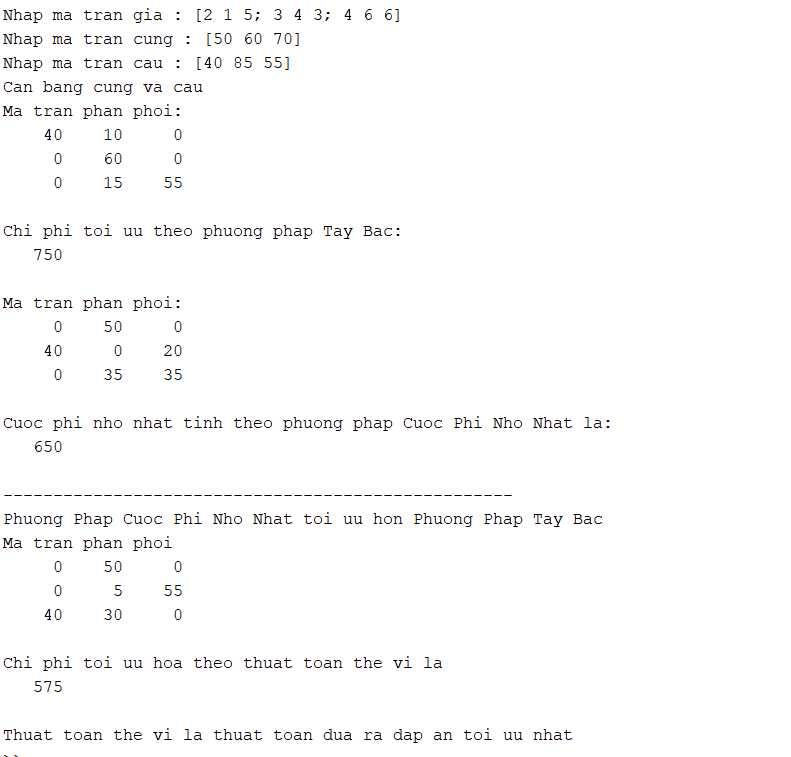
\includegraphics[scale=0.8, frame]{Images/code1.png}
    \caption{Kết quả thu được khi chạy chương trình}
    \label{fig:enter-label}
\end{figure}
\newpage
\begin{itemize}
    \item [$\square$] \textbf{Tiến hành kiểm tra lại kết quả.}
    \begin{itemize}[label=\textbullet]
        \item Ta lập được bảng sau:
    \end{itemize}
    \begin{table}[ht]
    \large
    \begin{center}
    \begin{tabular}{|l|w{c}{1.5cm}|w{c}{1.5cm}|w{c}{1.5cm}|l|} \hline
        Kho $(i)$ & \multicolumn{3}{c|}{Điểm bán lẻ $(j)$} & Tổng cung \\ \cline{2-4}
                  & 1    & 2   & 3      & \\ \hline 
        1         & $\text{\hspace{1.2cm}}^{2}$ & $\text{\hspace{1.2cm}}^{1}$ & $\text{\hspace{1.2cm}}^{5}$  & 50 \\  
                  &  & &  & \\ \hline
        2         & $\text{\hspace{1.2cm}}^{3}$ & $\text{\hspace{1.2cm}}^{4}$ & $\text{\hspace{1.2cm}}^{3}$  & 60 \\ 
                  &  &   &   & \\ \hline
        3         &  $\text{\hspace{1.2cm}}^{4}$ &$\text{\hspace{1.2cm}}^{6}$ &   $\text{\hspace{1.2cm}}^{6}$  &  \\ 
                  &  &   &   &70 \\ \hline
        Tổng cầu  &40 & 85 &  55   &  180\\ \hline
    \end{tabular}
    \end{center}
    \end{table}
    \item [$\square$] Theo phương pháp Tây Bắc
    \begin{itemize}[label=\textbullet]
        \item Chọn ô đầu tiên là ô $(i,j) = (1,1)$ làm ô xuất phát. Vì $d_1 = 40 < 50 = s_1$. Nên $x_{11} = 40$. Khi đó $s_1 = 50 - 40 = 10$.
        \item Chuyển qua ô tiếp theo $(i,j) = (1,2)$. Vì $s_1 = 10 < 85 = d_2$ nên $x_{12} = 10$. Khi đó $d_2 = 85 - 10 = 75$.
        \item Chuyển qua ô tiếp theo $(i,j) = (2,2)$. Vì $s_2 = 60 < 75 = d_2$ nên $x_{22} = 60$. Khi đó $d_2 = 75 - 60 = 15$.
        \item Chuyển qua ô tiếp theo $(i,j) = (3,2)$. Vì $d_2 = 15 < 70 = s_3$ nên $x_{32} = 15$. Khi đó $s_3 = 70 - 15 = 55$.
        \item Ta lập được bảng sau:
        \begin{table}[ht]
            \large
            \begin{center}
            \begin{tabular}{|l|w{c}{1.5cm}|w{c}{1.5cm}|w{c}{1.5cm}|l|} \hline
                Kho $(i)$ & \multicolumn{3}{c|}{Điểm bán lẻ $(j)$} & Tổng cung \\ \cline{2-4}
                          & 1    & 2   & 3      & \\ \hline 
                1         & $\text{\hspace{1.2cm}}^{2}$ & $\text{\hspace{1.2cm}}^{1}$ & $\text{\hspace{1.2cm}}^{5}$  & 50 \\  
                          & 40  & 10& $\boxed{ }$ & \\ \hline
                2         & $\text{\hspace{1.2cm}}^{3}$ & $\text{\hspace{1.2cm}}^{4}$ & $\text{\hspace{1.2cm}}^{3}$  & 60 \\ 
                          & $\boxed{ }$  &  60 & $\boxed{ }$   & \\ \hline
                3         &  $\text{\hspace{1.2cm}}^{4}$ &$\text{\hspace{1.2cm}}^{6}$ &   $\text{\hspace{1.2cm}}^{6}$  &  \\ 
                          & $\boxed{ }$  &  15 & 55  &70 \\ \hline
                Tổng cầu  &40 & 85 &  55   &  180\\ \hline
            \end{tabular}
            \end{center}
        \end{table}
    \end{itemize}
    \item [$\square$] Theo phương pháp cước phí nhỏ nhất
    \begin{itemize}[label = \textbullet]
        \item Chọn ô $(i,j) = (1,2)$ có cước phí nhỏ nhất là $c_{12}=1$. Vì $s_1 = 50 < 85 = d_2$ nên $x_{12} = 50$. Khi đó $d_2 = 85 - 50 = 30$. Loại hàng 1 vì hết khả năng cung cấp.
        \item Chọn ô $(i,j) = (2,1)$ có cước phí nhỏ nhất là $c_{21}= 3$. Vì $d_1 = 40 < 60 = s_2$ nên $x_{21} = 40$. Khi đó $s_2 = 60 - 40 = 20$. Loại cột 1 vì hết khả năng cung cấp.
        \item Chọn ô $(i,j) = (2,3)$ có cước phí nhỏ nhất là $c_{23}= 3$. Vì $s_2 = 20 < 55 = d_3$ nên $x_{23} = 20$. Khi đó $d_3 = 55 - 20 = 35$. Loại hàng 2 vì hết khả năng cung cấp.
        \item Từ các ô đã có suy ra được: $x_{32} = 35$ và $x_{33} = 35$.
        \item Ta lập được bảng sau:
    \end{itemize}
    \begin{table}[ht]
    \large
    \begin{center}
    \begin{tabular}{|l|w{c}{1.5cm}|w{c}{1.5cm}|w{c}{1.5cm}|l|} \hline
        Kho $(i)$ & \multicolumn{3}{c|}{Điểm bán lẻ $(j)$} & Tổng cung \\ \cline{2-4}
                  & 1    & 2   & 3      & \\ \hline 
        1         & $\text{\hspace{1.2cm}}^{2}$ & $\text{\hspace{1.2cm}}^{1}$ & $\text{\hspace{1.2cm}}^{5}$  & 50 \\  
                  & $\boxed{ }$ & 50& $\boxed{ }$ & \\ \hline
        2         & $\text{\hspace{1.2cm}}^{3}$ & $\text{\hspace{1.2cm}}^{4}$ & $\text{\hspace{1.2cm}}^{3}$  & 60 \\ 
                  & 40 &  $\boxed{ }$ & 20  & \\ \hline
        3         &  $\text{\hspace{1.2cm}}^{4}$ &$\text{\hspace{1.2cm}}^{6}$ &   $\text{\hspace{1.2cm}}^{6}$  &  \\ 
                  & $\boxed{ }$ & 35  & 35  &70 \\ \hline
        Tổng cầu  &40 & 85 &  55   &  180\\ \hline
    \end{tabular}
    \end{center}
    \end{table}
    \item [$\square$] Theo thuật toán thế vị:
    \begin{itemize}[label=\textbullet]
        \item Ta sẽ sử dụng phương án ban đầu là ma trận thu được ở phương pháp cước phí nhỏ nhất
        \item Chọn $u_1 = 0 \longrightarrow v_2 = 1 \longrightarrow u_3 = 5 \longrightarrow v_3 = 1 \longrightarrow u_2 = 2 \longrightarrow v_1 = 1$. 
        \item Tính các hệ số ước lượng: $\Delta_{11} = -1$; $\Delta_{13} = -4$;
        $\Delta_{22} = -1$; $\Delta_{31} = 2$. Còn lại bằng 0.
        \item Ta lập được bảng sau:
        \begin{table}[ht]
            \large
            \begin{center}
            \begin{tabular}{|l|w{c}{1.5cm}|w{c}{1.5cm}|w{c}{1.5cm}|l|w{c}{1.5cm}|} \hline
                Kho $(i)$ & \multicolumn{3}{c|}{Điểm bán lẻ $(j)$} & Tổng cung & $u_i$\\ \cline{2-4}
                          & 1    & 2   & 3      & &\\ \hline 
                1         & $\text{\hspace{1.2cm}}^{2}$ & $\text{\hspace{1.2cm}}^{1}$ & $\text{\hspace{1.2cm}}^{5}$  & 50 &\\  
                          & $\boxed{-1}$  & 50& $\boxed{-4}$ & & 0\\ \hline
                2         & $\text{\hspace{1.2cm}}^{3}$ & $\text{\hspace{1.2cm}}^{4}$ & $\text{\hspace{1.2cm}}^{3}$  & 60 &\\ 
                          & 40  &  $\boxed{-1}$ & 20 &  & 2\\ \hline
                3         &  $\text{\hspace{1.2cm}}^{4}$ &$\text{\hspace{1.2cm}}^{6}$ &   $\text{\hspace{1.2cm}}^{6}$ & &  \\ 
                          & $\boxed{+ 2}$  &  35 & 35  &70 & 5\\ \hline
                Tổng cầu  &40 & 85 &  55   &  180 & \\ \hline
                $v_j$  & 1 & 1 &  1   &   & \\ \hline
            \end{tabular}
            \end{center}
        \end{table}
        \item Chọn ô có hệ số ước lượng dương lớn nhất là $\Delta_{31} = 2$. Chọn các ô $x_{21}$; $x_{23}$; $x_{33}$. Giá trị nhỏ nhất của ô $x_{21}$ và $x_{33}$ là 35, loại ô $x_{33}$ khỏi bảng. Tăng ô $x_{31}$ và $x_{23}$ thêm 35 và giảm $x_{33}$ đi 35. Ta lập bảng mới với các thế vị và hệ số ước lượng mới.
        \item Chọn $u_1 = 0 \longrightarrow v_2 = 1 \longrightarrow u_3 = 5 \longrightarrow v_1 = -1 \longrightarrow u_2 = 4 \longrightarrow v_3 = -1$. 
        \item Tính các hệ số ước lượng: $\Delta_{11} = -3$; $\Delta_{13} = -6$;
        $\Delta_{22} = 1$; $\Delta_{33} = -2$. Còn lại bằng 0.
        \item Ta lập được bảng sau:
        \begin{table}[ht]
            \large
            \begin{center}
            \begin{tabular}{|l|w{c}{1.5cm}|w{c}{1.5cm}|w{c}{1.5cm}|l|w{c}{1.5cm}|} \hline
                Kho $(i)$ & \multicolumn{3}{c|}{Điểm bán lẻ $(j)$} & Tổng cung & $u_i$\\ \cline{2-4}
                          & 1    & 2   & 3      & &\\ \hline 
                1         & $\text{\hspace{1.2cm}}^{2}$ & $\text{\hspace{1.2cm}}^{1}$ & $\text{\hspace{1.2cm}}^{5}$  & 50 &\\  
                          & $\boxed{-3}$  & 50& $\boxed{-6}$ & & 0\\ \hline
                2         & $\text{\hspace{1.2cm}}^{3}$ & $\text{\hspace{1.2cm}}^{4}$ & $\text{\hspace{1.2cm}}^{3}$  & 60 &\\ 
                          & 5  &  $\boxed{+1}$ & 55 &  & 4\\ \hline
                3         &  $\text{\hspace{1.2cm}}^{4}$ &$\text{\hspace{1.2cm}}^{6}$ &   //////// & &  \\ 
                          & 35  &  35 &//////// &70 & 5\\ \hline
                Tổng cầu  &40 & 85 &  55   &  180 & \\ \hline
                $v_j$  & 1 & -1 &  1   &   & \\ \hline
            \end{tabular}
            \end{center}
        \end{table}
        \item Chọn ô có hệ số ước lượng dương lớn nhất là $\Delta_{22} = 1$. Chọn các ô $x_{21}$; $x_{31}$; $x_{32}$. Giá trị nhỏ nhất của ô $x_{21}$ và $x_{32}$ là 5, loại ô $x_{21}$ khỏi bảng. Tăng ô $x_{22}$ và $x_{31}$ thêm 5 và giảm $x_{33}$ đi 5. Ta lập bảng mới với các thế vị và hệ số ước lượng mới.
        \item Chọn $u_1 = 0 \longrightarrow v_2 = 1 \longrightarrow u_3 = 5 \longrightarrow v_1 = -1 \longrightarrow u_2 = 3 \longrightarrow v_3 = 0$. 
        \item Tính các hệ số ước lượng: $\Delta_{11} = -3$; $\Delta_{13} = -5$;
        $\Delta_{21} = -1$; $\Delta_{33} = -1$. Còn lại bằng 0.
        \item Ta lập được bảng sau:
        \begin{table}[ht]
            \large
            \begin{center}
            \begin{tabular}{|l|w{c}{1.5cm}|w{c}{1.5cm}|w{c}{1.5cm}|l|w{c}{1.5cm}|} \hline
                Kho $(i)$ & \multicolumn{3}{c|}{Điểm bán lẻ $(j)$} & Tổng cung & $u_i$\\ \cline{2-4}
                          & 1    & 2   & 3      & &\\ \hline 
                1         & $\text{\hspace{1.2cm}}^{2}$ & $\text{\hspace{1.2cm}}^{1}$ & $\text{\hspace{1.2cm}}^{5}$  & 50 &\\  
                          & $\boxed{-3}$  & 50& $\boxed{-6}$ & & 0\\ \hline
                2         & //////// & $\text{\hspace{1.2cm}}^{4}$ & $\text{\hspace{1.2cm}}^{3}$  & 60 &\\ 
                          & ////////  &  5 & 55 &  & 3\\ \hline
                3         &  $\text{\hspace{1.2cm}}^{4}$ &$\text{\hspace{1.2cm}}^{6}$ &   //////// & &  \\ 
                          & 40  &  30 &//////// &70 & 5\\ \hline
                Tổng cầu  &40 & 85 &  55   &  180 & \\ \hline
                $v_j$  & -1 & 1 &  0   &   & \\ \hline
            \end{tabular}
            \end{center}
        \end{table}
        \item Vì các hệ số ước lượng đều âm nên đây chính là phương án tối ưu của bài toán theo thuật toán thế vị. 
    \end{itemize}
    \item [$\square$] \textbf{Kết quả kiểm tra đúng theo đáp án của phần mềm.}
\end{itemize}
\newpage
\paragraph{Giá trị đầu vào thứ hai}
\begin{flushleft}
\hspace{0.4cm} Nhap ma tran gia: [1 2 4 3 ; 2 3 2 7 ; 3 5 6 4] \medskip \\
\hspace{0.4cm} Nhap ma tran cung: [60 70 20] \medskip \\
\hspace{0.4cm} Nhap ma tran cau: [30 40 30 50] \medskip \\
\hspace{0.4cm} Đây chính là giá trị đầu vào của bài toán được trình bày ở \textbf{\underline{Ví dụ}} \ref{fig:VD} trong thuật toán \textbf{Thế vị}
\end{flushleft}
\paragraph{Kết quả thu được:}
\begin{flushleft}
    \hspace{0.4cm}Kết quả thu được khi chạy chương trình
\end{flushleft}
\begin{figure}[ht]
    \centering
    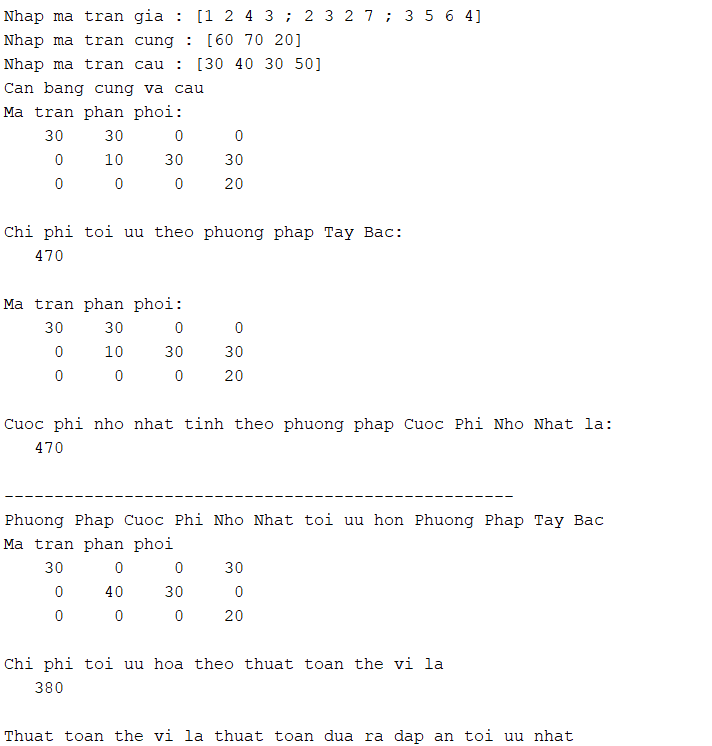
\includegraphics[scale=0.8, frame]{Images/code2.png}
    \caption{Kết quả thu được khi chạy chương trình}
    \label{fig:enter-label}
\end{figure}

\newpage
\section*{IV. Nguồn trích dẫn}
\addcontentsline{toc}{section}{\protect\numberline{}IV. Nguồn trích dẫn}
\setcounter{section}{1}\setlength{\baselineskip}{15pt}
   % đếm số cho section2, nếu không là hiện 0.1, 0.1.1
\setcounter{subsection}{0}
\setcounter{subsubsection}{0}
\label{sec:citations}
Trích dẫn \textit{et. al.} \cite{meyer2023matrix,anton2013elementary,amidror2013mastering,QuyHoachTuyenTinh,GiaoTrinhQuyHoachTuyenTinh}

\bibliographystyle{ieeetr}
\bibliography{refs}


\end{document}
